\documentclass{article}
\usepackage[utf8]{inputenc}
\usepackage[english]{babel}
\usepackage{apacite}
\usepackage{graphicx}
\usepackage{mathptmx}
\usepackage[font = {small, it}]{caption}
\DeclareCaptionLabelFormat{cont}{#1~#2\alph{ContinuedFloat}}
\captionsetup[ContinuedFloat]{labelformat=cont}
%\usepackage{subcaption}
\usepackage{subfigure}
\usepackage{float}
\usepackage{fancyhdr}
\usepackage{listings}

\lstset{language=Python}

%% CHANGE MARGINS

\addtolength{\oddsidemargin}{-.875in}
\addtolength{\evensidemargin}{-.875in}
\addtolength{\textwidth}{1.75in}

\addtolength{\topmargin}{-.875in}
\addtolength{\textheight}{1.75in}

%% make header

\fancypagestyle{plain}{
\fancyhf{}
\rhead{Mikkel Werling (201706722) \\
    Emil Rønn (201705177) \\
    Victor Møller Poulsen (201707639)}
\lhead{PyCipio}
\cfoot{\thepage}
}
\pagestyle{plain}

\setlength{\parindent}{2em}
\setlength{\parskip}{1em}
\renewcommand{\baselinestretch}{1.5}

\title{PyCipio: Bayesian Time-series Prediction}
\author{Mikkel Werling (201706722) \\
    Emil Rønn (201705177) \\
    Victor Møller Poulsen (201707639)}
\date{}
\begin{document}
\maketitle
\section{Abstract}
Several forecasting frameworks and packages are available for producing time series forecasts. However, these are typically based on frequentist statistics, or do not estimate the full posterior using Markov Chain Monte Carlo (MCMC). Here, we present PyCipio, a developmental, user-friendly python module that employs fourier series for time series decomposition, in conjunction with a Bayesian back-end for modelling and inference with the aim of propagating the full uncertainty forward into our predictions. The intended workflow of PyCipio is discussed and a demonstration across three different cases is used to highlight its strengths and limitations. Lastly, future avenues for improvement are discussed.     
\section{Introduction}
\subsection{Time Series Forecasting}

Time series forecasting revolves around predicting the future. Its use cases span fields such as commerce, marketing and economics, as well as several branches of science \cite{Chatfield}. Because of this multitude in applicability, time series forecasting is really an umbrella term covering a list of highly specialized methodologies, each aiming to solve specific forecasting tasks, often within specific domains. A time series consists of a variable storing time ($t$) which is used to predict some quantity of interest ($y$). The motivation behind time series forecasting is rooted in understanding the patterns of the past, their trends, periodicity, or volatility, with the hopes of predicting future events. From a business perspective, companies that can reliably predict their sales, expected production costs, and sick days in their workforce are better able to take preemptive measures and to thrive in a competitive market. Physicians and statisticians working in conjunction to build reliable models concerning health related issues, can help inform social policy and create meaningful public health responses. An example is offered by \citeA{dengue} who made use of a SARIMA model to implement a reliable 3 months-ahead early warning system for dengue fever outbreaks.

Four primary factors affect the quality of the forecasts that can be make of a time-series \cite{fpp3}:

\begin{itemize}
    \item How well we understand the factors that contribute to it;
    \item How much data is available;
    \item How similar the future is to the past;
    \item Whether the forecasts can affect the thing we are trying to forecast.
\end{itemize}

If we do not understand the factors that contribute to the development of a time-series, it can be hard to design good models in practise. However, we might still be able to design a model which can predict future data even if we do not understand the causal mechanisms. 

If there is only little data available, we can rely on “judgemental forecasts” \cite{fpp3}. Judgemental forecasts are constrained by the experiences, biases, and cognitive limitations brought on by the individual forecaster. A better approach might be to involve domain experts in designing models and setting informative priors for the forecast model.  This is possible in a Bayesian framework such as the one that we present.

If the future is dissimilar to the past or the forecast affects what we are trying to forecast then we might not be able to generate any reliable predictions. A case in which past patterns do not repeat in the future could be COVID cases which (as we will discover) do not contain a reliable and repeating signal. A case in which the forecasts of a system influence the system itself is election forecasts affecting voting behavior \cite{exit-polls1, exit-polls2,exit-polls3}. Our models can only extrapolate from the patterns they have already been exposed to. They cannot expect the unexpected. If the past gives us no reason to expect a particular change in the signal, predicting that change will be inherently out of our reach. 

Besides these factors the horizon of the forecast obviously influences the accuracy of predictions that we are able to generate. Long-term forecasts tend to be more volatile and subject to more uncertainty than short-term forecasts \cite{Luke-Muehlhauser}.  


\subsection{Decomposition of a Signal}

Real life time-series often have a number of features in common. Most time-series are influenced by multiple seasonal patterns (weekly, monthly, yearly), as well as an overall trend \cite{taylor2018forecasting}. For instance, global temperature can be modelled with a seasonal component as well as an upwards trend which could be either linear or exponential. Different techniques can be used to separate these components from each other in the time-series. This method of splitting the raw signal into different components is referred to as decomposition \cite{fpp3, taylor2018forecasting}. In our case, we decompose the signal into a trend component and two different seasonal components. Using decomposition for modelling time-series is often helpful in order to design an appropriate model and to facilitate interpretation of parameter estimates. It helps interpretability because one can analyze each component independently. Additionally it allows us to combine simple distributions to model a complex signal. It is flexible because we can add or remove a component without fundamentally changing the model \cite{taylor2018forecasting}. 

In the decomposition of a signal, we imagine the time-series being generated from a number of different components, which are added or multiplied to generate the data;

$$y(t) = g(t) + s(t) + \epsilon$$

\begin{center}
    or
\end{center}

$$y(t) = g(t) \cdot s(t) \cdot \epsilon $$

where $t$ is time, $y(t)$ is the actual raw signal, $g(t)$ is trend, $s(t)$ is the seasonal component and $\epsilon$ is the error term. 

The main difference between an additive and a multiplicative decomposition is how they interact with time. The additive component is best suited when the amplitude of the seasonal component does not vary as a function of time, but stays constant. Alternatively, when the amplitude changes over time, a multiplicative decomposition will be more appropriate. 

For our model, we conceptualize the trend component as a linear model with a slope ($\beta$) and an intercept ($\alpha$):

$$g(t) = \alpha + \beta \cdot x$$

Note that this gives equal weight to all data points in our training data. In most cases the most recent data points should probably have a higher weight than observations from the distant past. This is often achieved by exponentially discounting observations based on how far back in time they are \cite{gilchrist1967methods}. The consequence of this modeling choice is scrutinized in the second example which will be presented later.

We conceptualize the seasonal component as a Fourier series, a flexible way of modelling periodic effects \cite{taylor2018forecasting}. Fourier series rely on two inputs; the number of components ($N$) used to fit the seasonal tendency as well as the period of these components ($p$). If the data has daily measurements, a $p = 7$ would model a weekly seasonality, while a $p = 365.25$ would model a yearly seasonality. The Fourier series can model arbitrarily complex data, when $\lim_{N\to\infty} s(t)$ \cite{taylor2018forecasting}:

$$s(t) = \sum _{n=1} ^N \left( a_n cos(\frac{2 \pi n t}{P}) + b_n sin(\frac{2 \pi n t}{P}) \right)$$

Fourier series rely on estimating the $2N$ parameters, $\gamma = [a_1, b_1, … a_n, b_n]^T$. This can be done by constructing a matrix of these vectors for each $t$ in the training data. For $N = 8$ and $p = 7$:

$$F(t) = \left[ \cos(\frac{2 \pi 1 t}{7}), \sin(\frac{2 \pi 1 t}{7}) \dots, \cos(\frac{2 \pi 8 t}{7}), \sin(\frac{2 \pi 8 t}{7}) \right]$$

The seasonal component is then weighted by a parameter, $\omega$ so that:

$$s(t) = F(t) \cdot \omega$$

Increasing $N$ within a seasonal component allows for modelling quick changes in periodicity as well as more complex patterns. Increasing $N$ does run the risk of overfitting the model, and increasing it should be done with caution. In our current framework, we model two different seasonal components, which allows for modelling for instance a yearly and a weekly trend. These two seasonal components are independent. $N$, $p$ and whether they are additive or multiplicative can be specified differently for the two components. In sum, our model specification is as follows for the additive case:

$$y(t) = \alpha + \beta \cdot x + s_1(t) + s_2(t)$$

where a multiplicative seasonal component would be achieved by simply multiplying a seasonal component with $t$, i.e. $(s_n(t) \cdot t)$.


\subsection{Bayesian Framework}

There are several good packages available for time series forecasting in a variety of programming languages. For instance, R has the excellent fable and feasts packages \cite{fable_package, feasts_package} as used in fpp3 \cite{fpp3}, and scikit-learn \cite{scikit-learn} is a good option for users working in Python. However, most packages suited for easy time-series forecasting are, to our knowledge, based on frequentist statistics. We propose PyCipio as an alternative for the users who want the easy workflow from these packages, but prefer a Bayesian analysis.   

In Bayesian statistics, we provide assumptions about the data generating process in the form of probability distributions for parameters and we specify how these parameters should be combined to produce data in the form of a likelihood function. Bayes theorem is then used to optimally estimate our parameters given our data \cite[p.~9]{martin2018bayesian}.

The Bayesian framework offers a host of advantages as compared to a frequentist framework.

Firstly, a full posterior estimation with Markov Chain Monte Carlo (MCMC) is superior to quadratic approximation, which is often used in frequentist statistics. It is also superior to Bayesian Maximum A Posteriori (MAP) estimation which is the default option in Facebook Prophet \cite{taylor2018forecasting}. This is especially true if the posterior distribution is not well approximated by a multivariate Gaussian distribution (e.g. if the mode and the mean are not the same) \cite[p.~325]{McElreath}.

Secondly, Bayesian models are always generative. This is the case because the likelihood function allows us to run the model both “forwards” and “backwards”. Given observations, a likelihood function tells us how plausible these observations are. We can perform backwards inference to estimate plausible distributions for the parameters generating this data.  Given parameters, the likelihood function defines a distribution of plausible outcomes that we can sample from \cite[p.~62]{McElreath}. As such, we run our model “backwards” when we infer parameters given data, and then we run the model “forward” when we generate new data based on these parameters and our likelihood function.

This is useful, because we can then obtain simulations (predictions) from our model which incorporate all the uncertainty of both our observations and our parameters. Since we are not simply computing point estimates for our parameters, but estimate the full distributions of plausible parameter values, we can propagate the “honest” uncertainty forward in our predictions (\citeNP[p.~64]{McElreath}, \citeNP[p.~1]{gelman2020bayesian}). The figure (below), which is taken from \cite[p.~65]{McElreath}, illustrates this nicely. At the top we see an estimated posterior distribution (over the amount of water on earth). We can then draw samples from the posterior and each of these samples will have an associated sampling distribution (here the likelihood is binomial). This is then combined in the posterior predictive distribution, which incorporates the uncertainty of all the levels of analysis.


\begin{figure}[H]
    \centerline{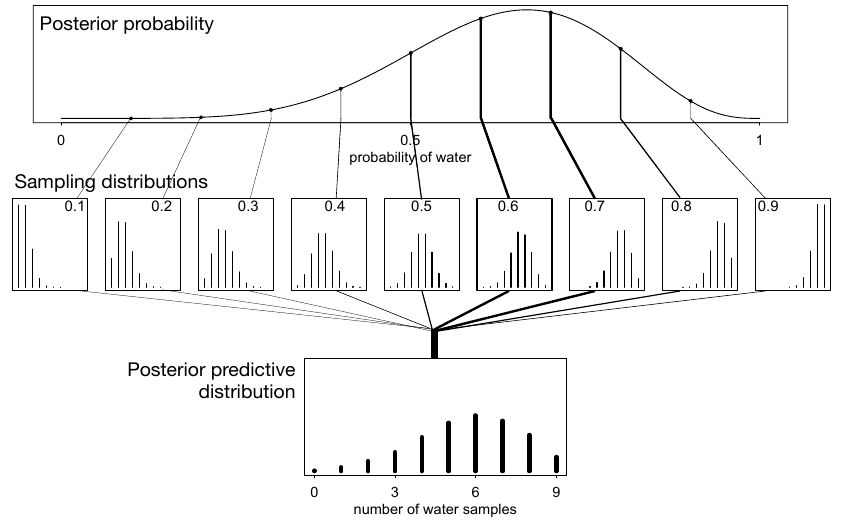
\includegraphics[scale = 0.5]{images/McElreath.png}}
    \caption{(taken from McElreath, p. 65). (top row) the posterior distribution over the amount of water on earth given a number of samples of either “water” or “earth”. We can sample parameter values from this posterior proportional to the density of the distribution, and each of these values will have an associated sampling distribution (middle row). Since “p” is the probability of water on each observation, there will still be uncertainty about observations, even if we are certain about p. We thus have both parameter uncertainty (uncertainty with regards to p) and uncertainty with regards to our observation realization. Both these levels of uncertainty are propagated forward to the posterior predictive distribution (bottom)}
\end{figure}

This naturally leads to the most obvious drawback of using a Bayesian framework, both generally, and for time-series forecasting. Because we want to estimate distributions for all our parameters, Bayesian models are computationally expensive to fit and sample from \cite[p.~13]{McElreath}. They might also be more expensive in terms of labor, because it can be necessary to think and tweak iteratively to specify reasonable priors and build sensible models.

While Bayesian models can be tricky to work with, we believe that it is an advantage that the user is required to specify priors for their model. This facilitates the incorporation of domain knowledge into the modeling context. If domain experts have reason to believe that there should be a weekly seasonal component in the data that they are attempting to forecast, then it should be possible to incorporate this information into the model. This knowledge of course needs to be translated into a mathematical specification (i.e. the expert needs to quantify their level of certainty). Even if the (training) data does not fully support such a trend, it might be a better (or more generalizable) model than one which simply finds the best fit to training data. 

\section{Implementation and Architecture}

\subsection{Object Oriented Programming}

The PyCipio codebase was written in Python \cite{Rossum}. Python is a multi-paradigm language, which supports both functional and object oriented programming. The difference between the two programming paradigms is whether the functionality of the script comes from pure functions, or from methods in an object. Although a functional programming implementation could have been used for PyCipio, we chose to opt for an object oriented solution. In Python, this is done by building what is called a "class". A class acts as a container for both the different data objects (attributes) and different methods which act upon the data (methods). Using an object oriented solution was done primarily for ease of use, convention in related packages and to ensure that the format of the data was consistent throughout the process.

One of main advantages of popular machine learning packages in Python (i.e. scikit-learn) is how easy they are to use \cite{Hao}. In most use-cases, only the data and the choice of model needs to be supplied by the user. The reason for this ease of use comes largely from their implementation as a class, where the object is initialized with the necessary values and manipulates them appropriately. The workflow in packages such as scikit-learn for getting predictions on unseen data is as easy as initializing the object, using its ".fit()"-method, and finally using its ".predict()"-method. 

\begin{figure}[H]
    \centerline{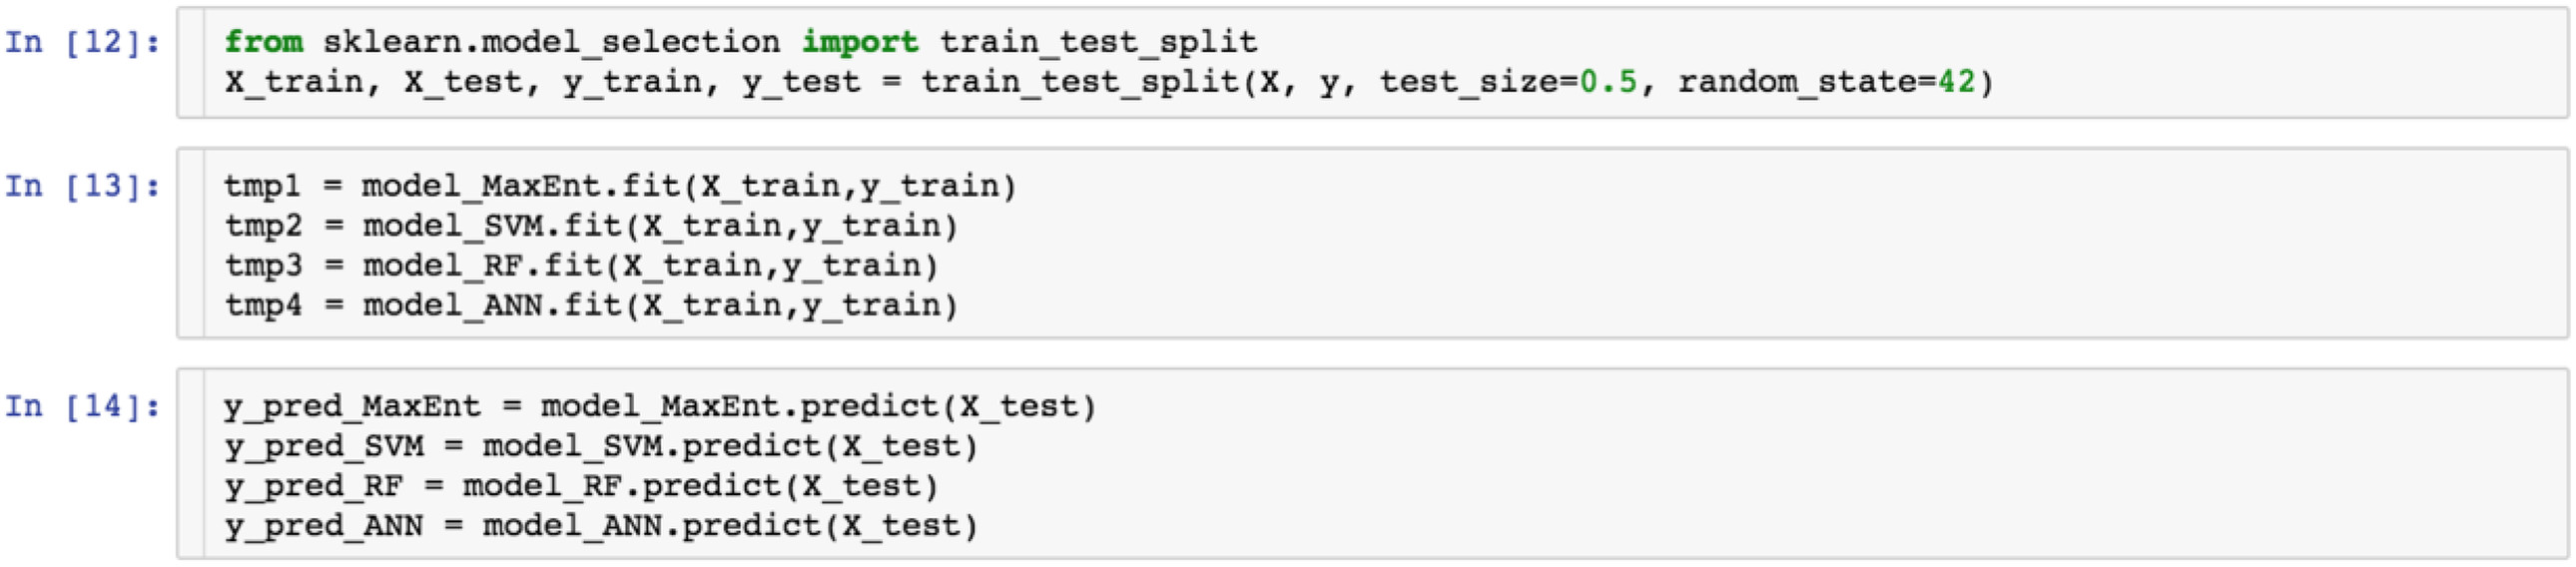
\includegraphics{images/sklearn.jpeg}}
    \caption{Taken from (Hao \& Ho, 2019). Showing a minimal scikit-learn pipeline for generating predictions. First cell imports the package and splits the data into training and test data. Second cell fits a number of models to the training data, and the last cell generates predictions on unseen data from these models. }
\end{figure}

As our software is designed to make time-series forecasting, we wanted to make sure that generating predictions for unseen data was as easy as it is in sklearn. However, the backend we are using for modelling and inference (PyMC3) is not user friendly when it comes to generating predictions specifically for time series decomposition. (looping is natural for decomposition, but we need to vectorize it. Not user friendly) The reason for this is primarily that the decompositions need to be vectorized as they rely on mathematical operations that only make sense if the dimensions match (for instance in terms of matrix multiplication). This is another point where object oriented programming is a better solution than functional programming in our case. By implementing PyCipio as an object, we can ensure that the training and the test data are matching in relevant dimensions. 

\subsection{Primary Functions}

Here we present the main methods which are implemented in the class, including which arguments they take and examples of how to use these methods. Here we only present some key functions. For a full overview consult the documentation at PyCipio’s Github: https://github.com/PyCipio/PyCipio (Github or the actual class: NB!! add readme)

\hrule

\begin{lstlisting}[language=Python]
PyCipio.__init__(data, time, values, index = None, split = 0.7):
\end{lstlisting}

\indent \textbf{Description:} 

\indent \indent Initializing the class. Assumes that data is a pandas DataFrame object.

\indent \textbf{Arguments:}

\indent \indent \textit{data (pd.DataFrame):} 

\indent \indent \indent Dataframe containing a column containing time indices and a column containing values. 

\indent \indent \indent Additionally, data can also contain a column which specifies groups in the data, but is not required. 

\indent \indent \textit{time (str):} 

\indent \indent \indent Column name in data, which specifies time indices.

\indent \indent \textit{values (str):} 

\indent \indent \indent Column name in data, which specifies the values of y.
            
\indent \indent \textit{index (str, optional):} 

\indent \indent \indent Column name in data, which specifies a grouping variable. If this variable is given, 

\indent \indent \indent the analysis will be carried out independently for each grouping. Defaults to None.

\indent \indent \textit{split (float, optional):} 

\indent \indent \indent Float indicating the proportion of data used for training. Defaults to 0.7.


\indent \textbf{Example:}
\begin{lstlisting}[language=Python]
		 Pc = PyCipio(data = data, 
                      time = "x", 
                      values = "y", 
                      index = "group", 
                      split = 0.8)

\end{lstlisting}

%%% FUNCTION 2
\hrule

\begin{lstlisting}[language=Python]
    PyCipio.fit(p1, p2, p1_mode, p2_mode, divisor = 20, deviation = 0.2):
\end{lstlisting}

\indent \textbf{Description:} 

\indent \indent Fits the model and plots the prior predictive distribution.

\indent \textbf{Arguments:}

\indent \indent \textit{p1 (tuple):} 

\indent \indent \indent Tuple of integers, where the first value is the value of p and the second value

\indent \indent \indent is the number of components. First value can be specified as a float, 

\indent \indent \indent while the second value must be an integer.

\indent \indent \textit{p2 (tuple):} 

\indent \indent \indent Tuple of integers, where the first value is the value of p and the second value

\indent \indent \indent is the number of components. First value can be specified as a float, 

\indent \indent \indent while the second value must be an integer.

\indent \indent \textit{p1\_mode (str):} 

\indent \indent \indent String indicating whether the seasonal component should be
multiplicative or additive. 

\indent \indent \indent If anything else than "multiplicative" is specified,
the mode defaults to additive.

\indent \indent \textit{p2\_mode (str):} 

\indent \indent \indent String indicating whether the seasonal component should be
multiplicative or additive. 

\indent \indent \indent If anything else than "multiplicative" is specified,
the mode defaults to additive.

\indent \indent \textit{divisor (int, optional):} 

\indent \indent \indent A scaling parameter for adjusting the standard deviation of the distribution
of p. 

\indent \indent \indent The standard deviation of p is set to p/divisor. Defaults to 20. 

\indent \indent \textit{deviation (float, optional):} 

\indent \indent \indent Parameter specifying the standard deviation of the beta for the seasonal
component. Defaults to 0.2.

\indent \textbf{Example:}

\begin{lstlisting}[language=Python]
        Pc.fit(p1 = (7, 2), 
            p2 = (365.25, 2), 
            p1_mode = "additive", 
            p2_mode = "multiplicative", 
            divisor = 15, 
            deviation = 0.3)    
\end{lstlisting}

%%% FUNCTION 3

\hrule

\begin{lstlisting}[language=Python]
    PyCipio.sample_mod(posterior_draws = 2000, post_pred_draws = 1000, 
    prior_pred_draws = 1000, random_seed = 42, chains = 2):
\end{lstlisting}

\indent \textbf{Description:} 

\indent \indent Sample the posterior, the posterior predictive, the prior predictive distribution and generate 

\indent \indent predictions on the test data.

\indent \textbf{Arguments:}

\indent \indent \textit{posterior\_draws (int, optional):} 

\indent \indent \indent Number of draws for the posterior. Defaults to 2000.

\indent \indent \textit{prior\_pred\_draws (int, optional):} 

\indent \indent \indent Number of draws for the prior predictive distribution. Defaults to 1000.

\indent \indent \textit{random\_seed (int, optional):}

\indent \indent \indent Random seed for ensuring reproducibility. Defaults to 42.

\indent \indent \textit{chains (int, optional):} 

\indent \indent \indent Number of chains used for sampling the posterior. Defaults to 2.

\indent \textbf{Example:}

\begin{lstlisting}[language=Python]
        Pc.sample_mod(posterior_draws = 3000, 
        post_pred_draws = 1500, 
        prior_pred_draws = 1500, 
        random_seed = 13, 
        chains = 4)
\end{lstlisting}

%%% FUNCTION 4

\hrule

\begin{lstlisting}[language=Python]
    PyCipio.plot_fit_idx(idx = None, path = False):
\end{lstlisting}

\indent \textbf{Description:} 

\indent \indent Plots the posterior predictive distribution overlayed on the training data.

\indent \textbf{Arguments:}

\indent \indent \textit{idx (list, optional):} 

\indent \indent \indent List of strings containing the names of the groups to plot. Defaults to None.

\indent \indent \textit{path (str, optional):}

\indent \indent \indent String specifying the path for saving the plot. 

\indent \indent \indent File-extension is automatically inserted and is hard set to .png. Defaults to False.

\indent \textbf{Example:}

\begin{lstlisting}[language=Python]
        Pc.plot_fit_idx(idx = ["group1", "group2"], path = "my_path/my_plot")
\end{lstlisting}

\noindent \textbf{Note:}

\noindent The same functionality exists for plotting the posterior predictive distribution overlayed on the training data. This method called \textit{plot\_prediction\_idx} is identical in inputs and outputs, but only differs on this point. For more details, see the full docstrings on Github. 

%%% FUNCTION 5

\hrule

\begin{lstlisting}[language=Python]
    PyCipio.plot_residuals(idx = None, path = False):
\end{lstlisting}

\indent \textbf{Description:} 

\indent \indent Plots the residuals from predictions generated by the model.

\indent \textbf{Arguments:}

\indent \indent \textit{idx (list, optional):}

\indent \indent \indent List of strings containing the names of the groups to plot. Defaults to None.

\indent \indent \textit{path (str, optional):}

\indent \indent \indent String specifying the path for saving the plot. 

\indent \indent \indent File-extension is automatically inserted and is hard set to .png. Defaults to False.

\indent \textbf{Example:}

\begin{lstlisting}[language=Python]
        Pc.plot_residuals(idx = ["group1", "group2"], path = "my_path/my_plot")
\end{lstlisting}

\subsection{Bayesian Modelling Workflow}

This section explains the intended usage and workflow of PyCipio. 

\begin{figure}[H]
    \centerline{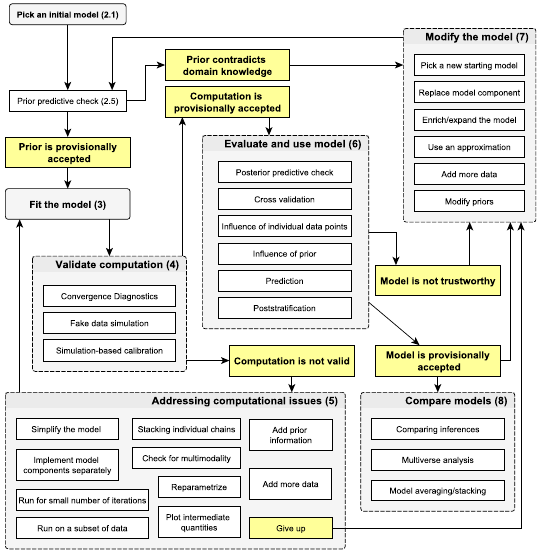
\includegraphics[scale = 0.5]{images/Gelman.png}}
    \caption{Taken from Gelman (2020, p. 5). Overview of the Bayesian workflow presented in Gelman (...). The numbers refer to pages in Gelman (...) and as such are not relevant here. The workflow starts to the top left with specifying an initial model and obtaining prior predictive checks, and ends with model comparison. Our modeling workflow stops at prediction. }
\end{figure}

Step 1: The user has to provide a pandas DataFrame object with at least two columns, one containing timepoints and one containing the corresponding outcome values. If the user wants to run the analysis on several clusters of data at once (e.g. on several companies, stocks or states) then an additional column is required which contains the id of the group that each observation belongs to. The data is then split into a train and test set. The default value for the split is 70\% train and 30\% test which is in the typical range \cite{Brownlee}. However, the user can choose other values if they so please.

Now the modeling workflow starts. Our intended usage is close to what is proposed by \citeA{gelman2020bayesian} and schematically shown below. In the places where it diverges from his workflow, this has been done purposefully because he is mainly focused on inference (i.e. parameter estimation) while we are exclusively interested in prediction. Notice that the workflow in several places is iterative rather than linear.

Step 2: The user specifies priors for the periods, for the number of components they want in each period, and whether the seasonal components should be additive or multiplicative. The priors for other values (e.g. intercept and linear trend) are set to broad and reasonable values at present and cannot be modified by the user in the current framework. Ideally it would be possible for the user to specify priors for all parameters without compromising the user friendliness. This step corresponds to the first step in the figure above, i.e. “Pick an initial model”. 

Step 3: Now the user can compile the model, which will automatically return a prior predictive check. Running a prior predictive check can be done before sampling the full posterior and is much faster. It thus makes sense to check that the priors that the user has specified (and the likelihood function which cannot be specified by the user) generates data that is on a reasonable scale as compared to the true posterior before investing time in fitting the model.

Step 3.1: If the prior predictive check is not satisfactory, then go back to step 2 and specify new priors. If the prior predictive check is satisfactory then proceed. This, again, corresponds to the figure above.

Step 4: The user will now fit the model, and at this step we generate prior predictive checks, posterior predictive checks and predictions on test data as well. 

Step 5:  The user should now validate that the sampling of the model was successful. This is aided by several plotting functionalities. Firstly, the user should generate a trace plot to verify that the chains look healthy, and that the parameters (distributions) look reasonable. Additionally, PyMC3 will flag issues such as divergences and poor mixing of chains (r-hat) for the user. Then the user should inspect the plot which shows both the prior-, and posterior predictive checks to verify that the model has learned appropriately from the data and that the posterior predictive fits the actual data much tighter than the prior predictive. The user should then check how well the mean posterior predictions fit the training data, and whether the uncertainty around these predictions is reasonable. 

Step 5.1: If any of these three diagnostic tools are unsatisfactory, then the user should return to step 2 and specify new priors for the model. Otherwise, the user should proceed. This step corresponds to “Validate computation” and “Evaluate and use model” in the Gelman figure.

Step 6: The user should now visualize predictions for the unseen test data. The user can also access several residual plots and forecast error indices (i.e. RMSE, MAE, MAPE, sMAPE). If residual plots show either (a) errors that are not distributed with mean 0 or (b) patterns in the residuals over time, then this strongly indicates that there is systematic variation in the data that the model is not capturing \cite{fpp3}. In this case the user could return to step 2. Otherwise the user should use these predictions for their intended purpose. 

This concludes the pipeline and intended workflow for time-series forecasting using PyCipio. Notice that there are several places (e.g. step 3, 5 and 6) where the user should return to earlier steps and iteratively improve on the model if diagnostics are not satisfactory. It often takes a lot of experimentation and iterative tweaking to properly fit complex Bayesian models (\citeNP[p.~1, p.~7]{gelman2020bayesian}, \citeNP[p.~9]{martin2018bayesian}). Also notice that we do not facilitate, or focus on presenting parameter estimation. The only place where the user will directly look at parameters is in the trace plot. Here the point is to verify that computation (sampling) has worked properly. 

\section{Examples}

In this section we present three example analyses showcasing useful features and limitations of PyCipio. All of the analyses are generated using almost exactly the same code pipeline. The first example will be the most thorough, showing almost all steps of the workflow, while the two following examples will only highlight the most interesting parts of the analysis. The general pipeline which all the analyses follow is shown below: 

\lstset{frame=lines}

\begin{lstlisting}
    #prep data (pandas dataframe containing a time series)
    d = pd.DataFrame(data)
    
    ##### create class ######
    Pc = pc.PyCipio(d, time = "time_column", 
                    values = "y_values", 
                    index = "idx_column", 
                    split = 0.7)
    
    ##### fit model: 
    Pc.fit(p1 = (7, 1), 
        p2 = (30, 1), 
        p1_mode = "multiplicative", 
        p2_mode = "additive")
    
    ##### sample #####
    Pc.sample_mod()
    
    ##### plotting #####
    Pc.plot_trace()
    Pc.plot_pp()
    
    ### plot training ###
    Pc.plot_fit_idx(idx = ["group 1", "group 2"])
    
    ### plot predict ###
    Pc.plot_predict_idx(idx = ["group 1", "group 2"])
    
    ### get errors ###
    Pc.get_errors()
    
    ### plot residuals ###
    Pc.plot_residuals(idx = ["group 1", "group 2"])
    
    ### save idata ### - This is if you want to save your model for later use
    Pc.save_idata()
\end{lstlisting}


\subsection{Example 1}

The first example of the pipeline/workflow is done on simulated data, in order to have something that is relatively clean and easy to understand. Here we aim to showcase a workflow on the kind of data that is currently well fitted and predicted by the model implemented in PyCipio and also showcase some of the issues that users might run into. 

The data used in this example consists of two time-series which are both simulated using four sine waves, four cosine waves, an intercept and a linear trend. The sine-, and cosine-waves both share the feature that the oscillations have periods of approximately 3.5, 7, 15 and 30 time points. The oscillation with period 3.5 will be nested twice within the oscillation with period 7, and the oscillation with period 15 will be nested twice within the oscillation with period 30. The intercepts and linear trends differ for the two time-series, and normally distributed errors are added for all components. 

\begin{figure}[H]
    \centerline{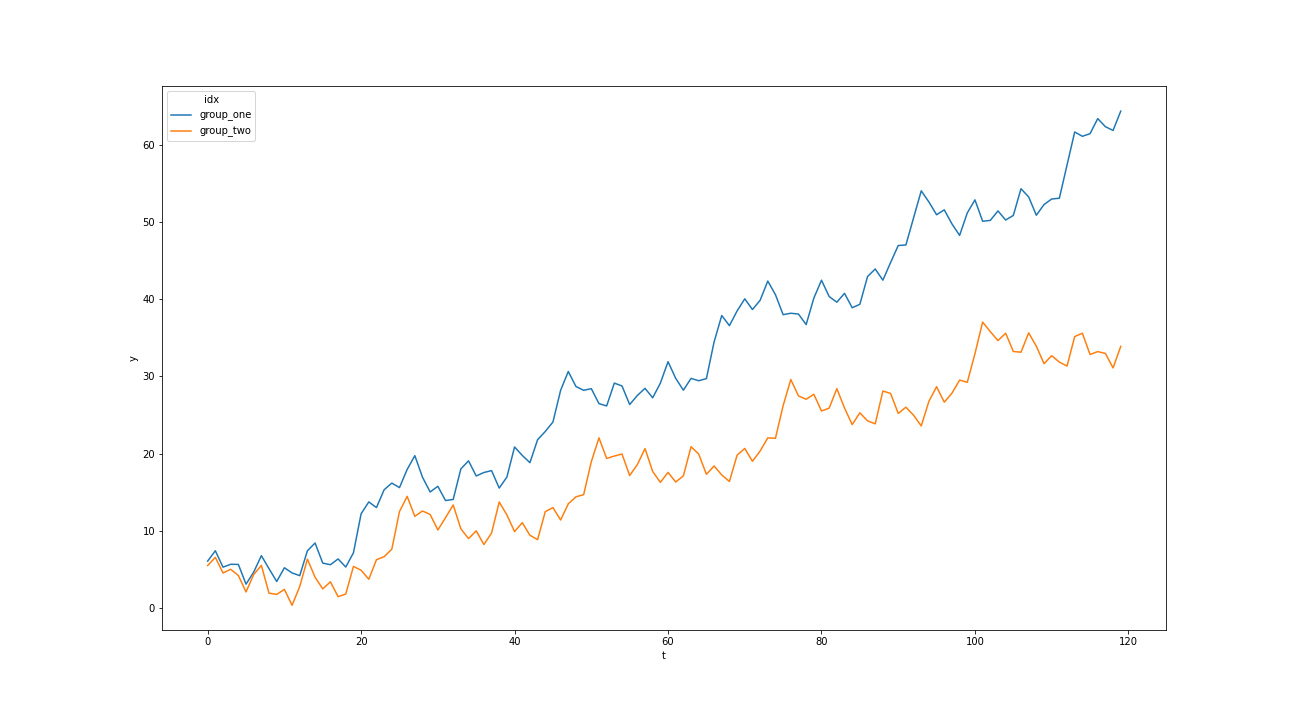
\includegraphics[scale = 0.45]{../plots/ex1_plot_data.png}}
    \caption{Seaborn line plot of the two simulated time-series. Generated with the plot\_data() method from PyCipio.}
\end{figure}

It is to be expected that we should be able to model this data well with an intercept, a linear component and two Fourier series which both have two components ($N$) and are approximately 7 and 30 timesteps long ($p$). It should be underfit (i.e. miss some of the seasonality) with two Fourier series which both have $N = 1$ and overfit with two Fourier series which both have $N = 5$. We will refer to the model with one component as model 1 (M1), the one with two components as model 2 (M2) and the one with five components as model 3 (M3).

After fitting the models, the first thing we will want to assess is the trace plots. Here we see that the parameters have been estimated without errors or reasons to worry for both M1 and M2. The associated traces (A, B) also show good mixing between the chains and have similar estimations for the distributions of the parameters. We note that the trace plot is problematic for M3 (C). Specifically, we see that the two chains have estimated our parameters very differently.

\begin{figure}[H]
    \centering
    \subfigure[M1]{%
        \label{fig:supfigure1}
        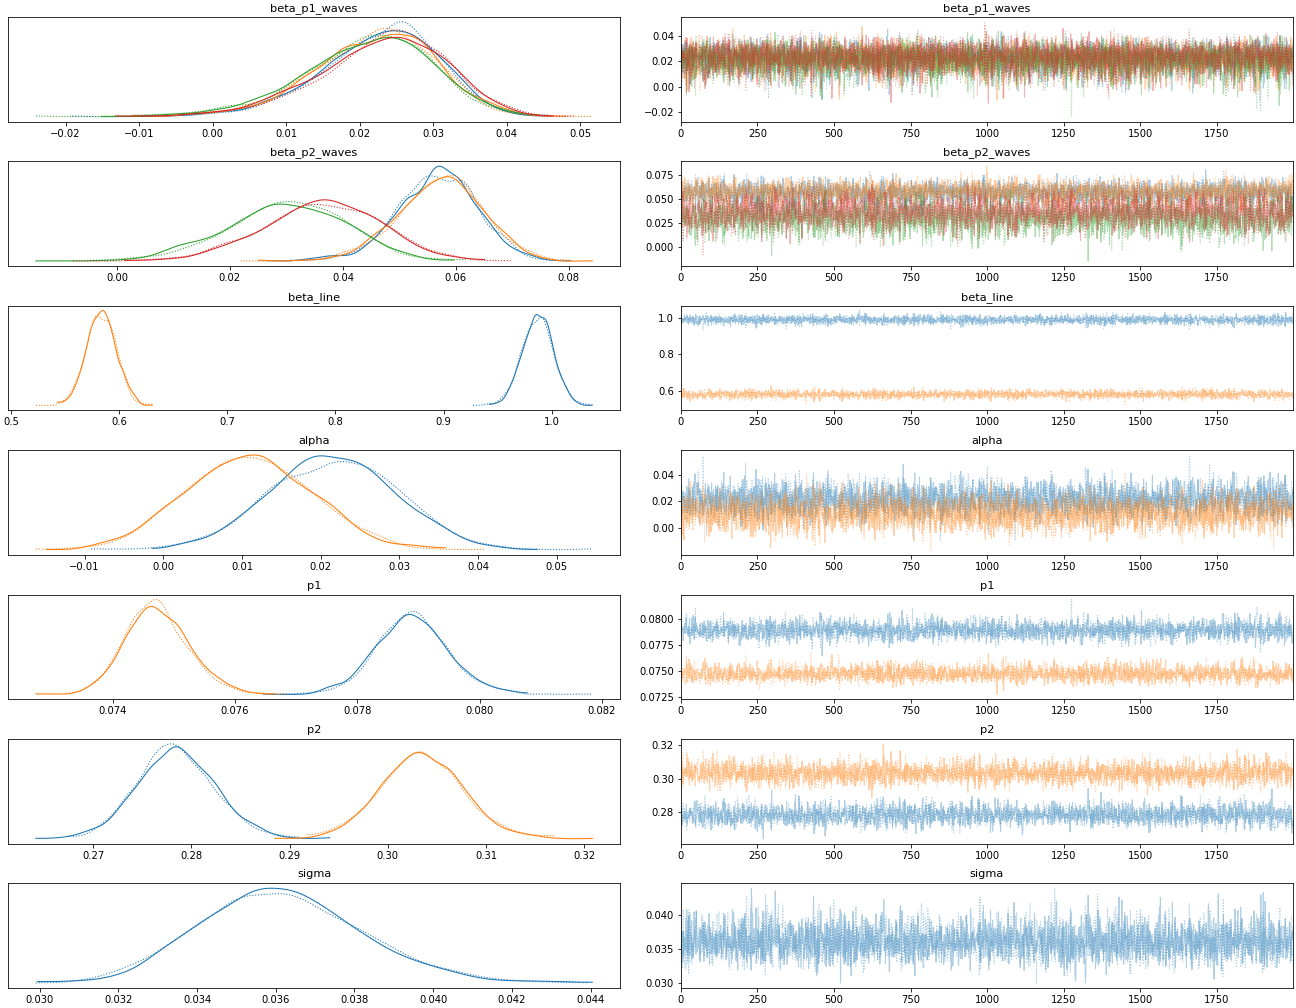
\includegraphics[width = 0.30 \textwidth]{../plots/ex1_first_plot_trace.png}}
    \quad
    \subfigure[M2]{%
        \label{fig:supfigure2}
        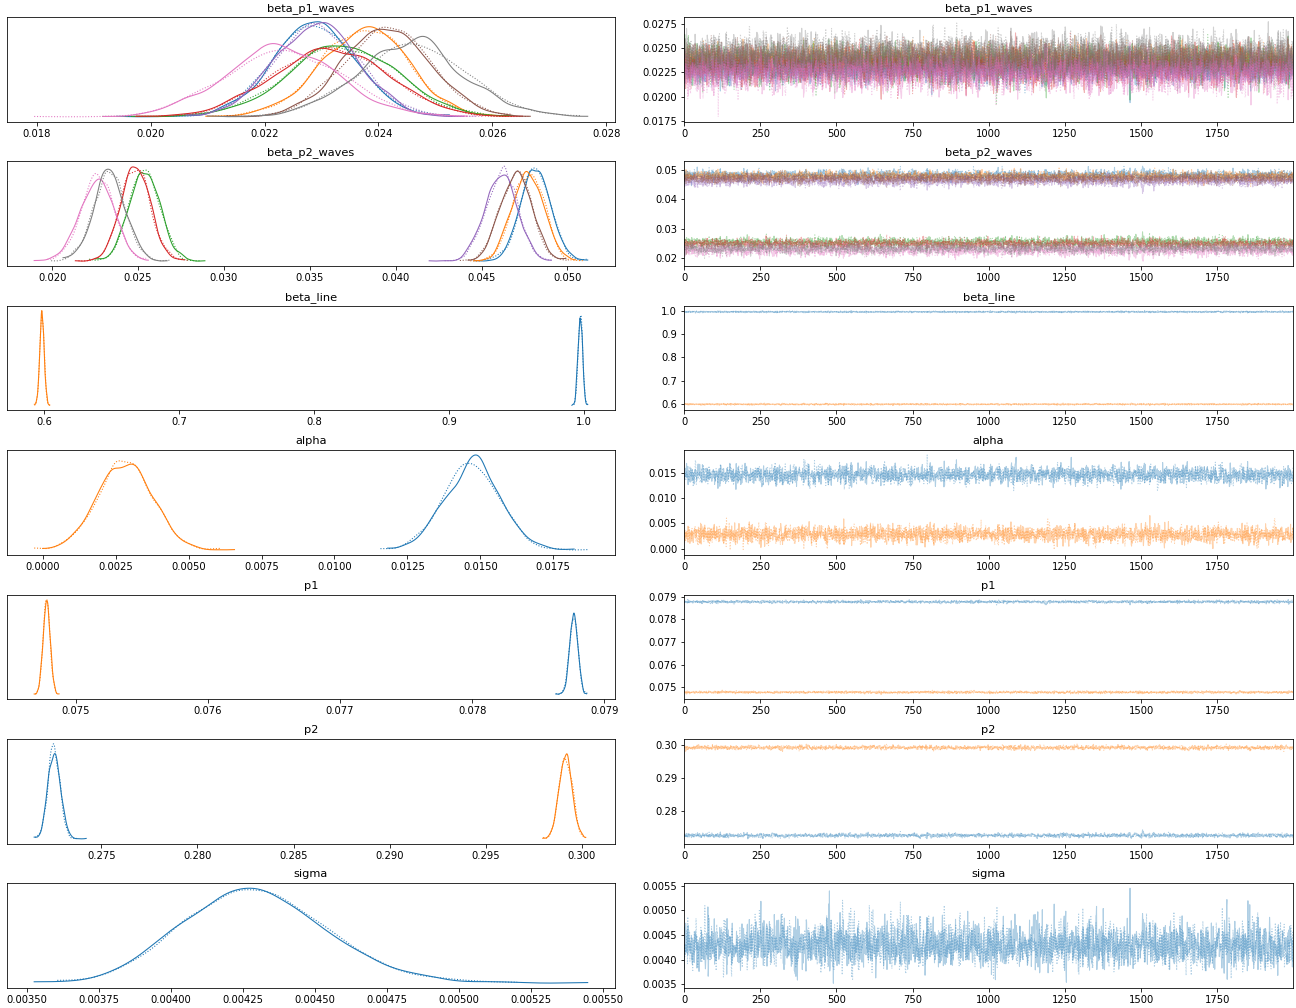
\includegraphics[width = 0.30 \textwidth]{../plots/ex1_second_plot_trace.png}}
    \subfigure[M3]{%
        \label{fig:supfigure3}
        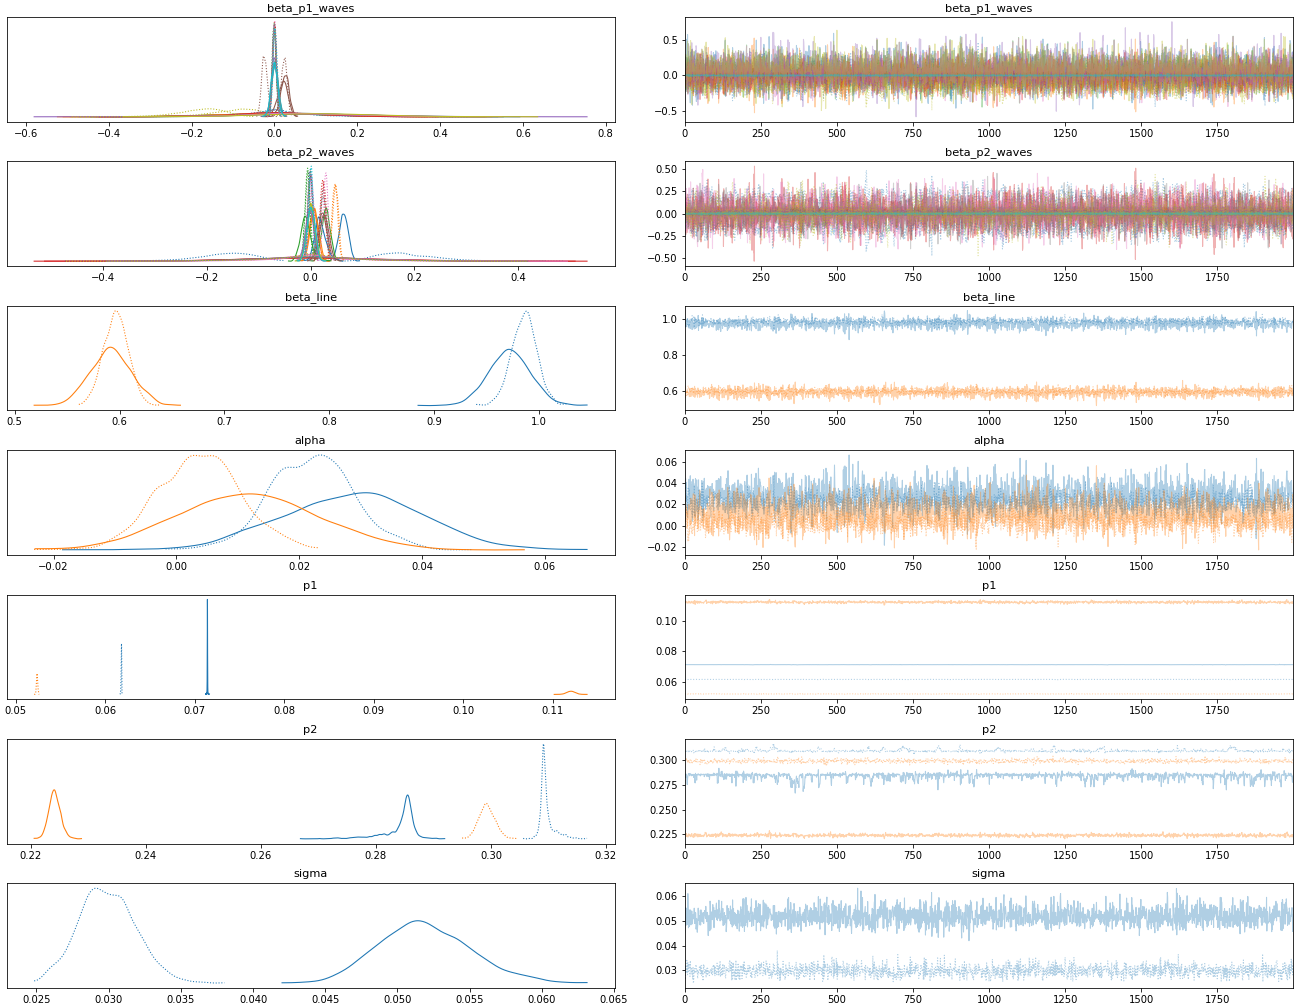
\includegraphics[width = 0.30 \textwidth]{../plots/ex1_third_plot_trace.png}}
    \quad
    \caption{Arviz trace plots for the three models (M1, M2, M3) from left to right. Generated by PyCipio's plot\_trace() method.}
\end{figure}

Continuing with all three models, we now inspect the prior- and posterior predictive plots. These indicate whether the model has learned from the data (i.e. updated our prior to fit the data). We see that the fit is not perfect for M1. This is to be expected since we do not have enough fourier components to fit a signal with our generative process. We see that the fit is almost perfect for M2. It is reassuring that our model can indeed decompose and fit this kind of signal. Again, we see that M3 is problematic, or at least that the posterior predictive fit is worse than for the model which is underfit (M1). 

\begin{figure}[H]
    \centering
    \subfigure[M1]{%
        \label{fig:supfigure1}
        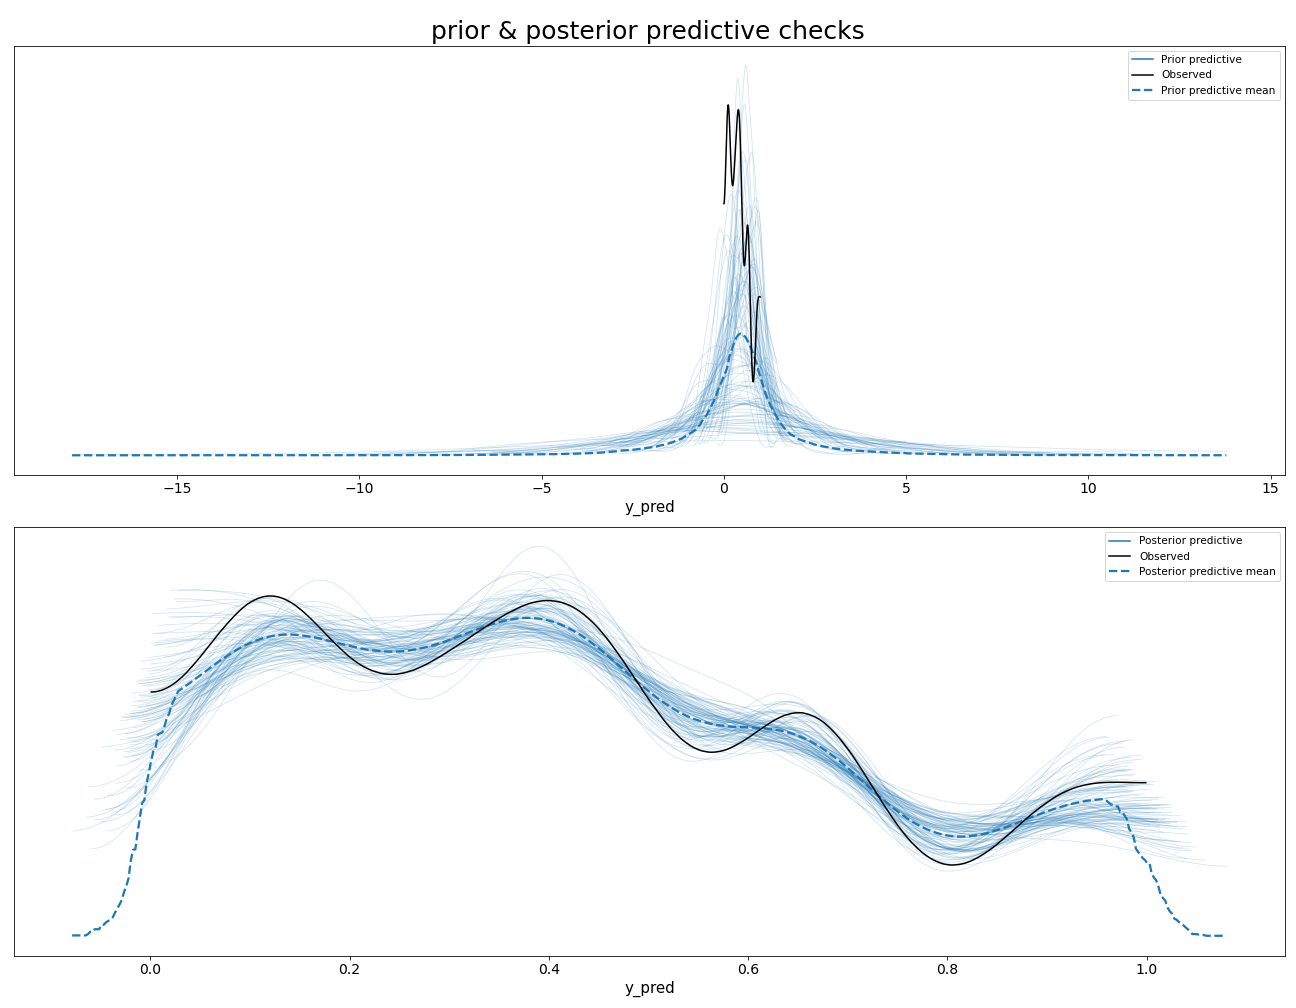
\includegraphics[width = 0.30 \textwidth]{../plots/ex1_first_plot_pp.png}}
    \quad
    \subfigure[M2]{%
        \label{fig:supfigure2}
        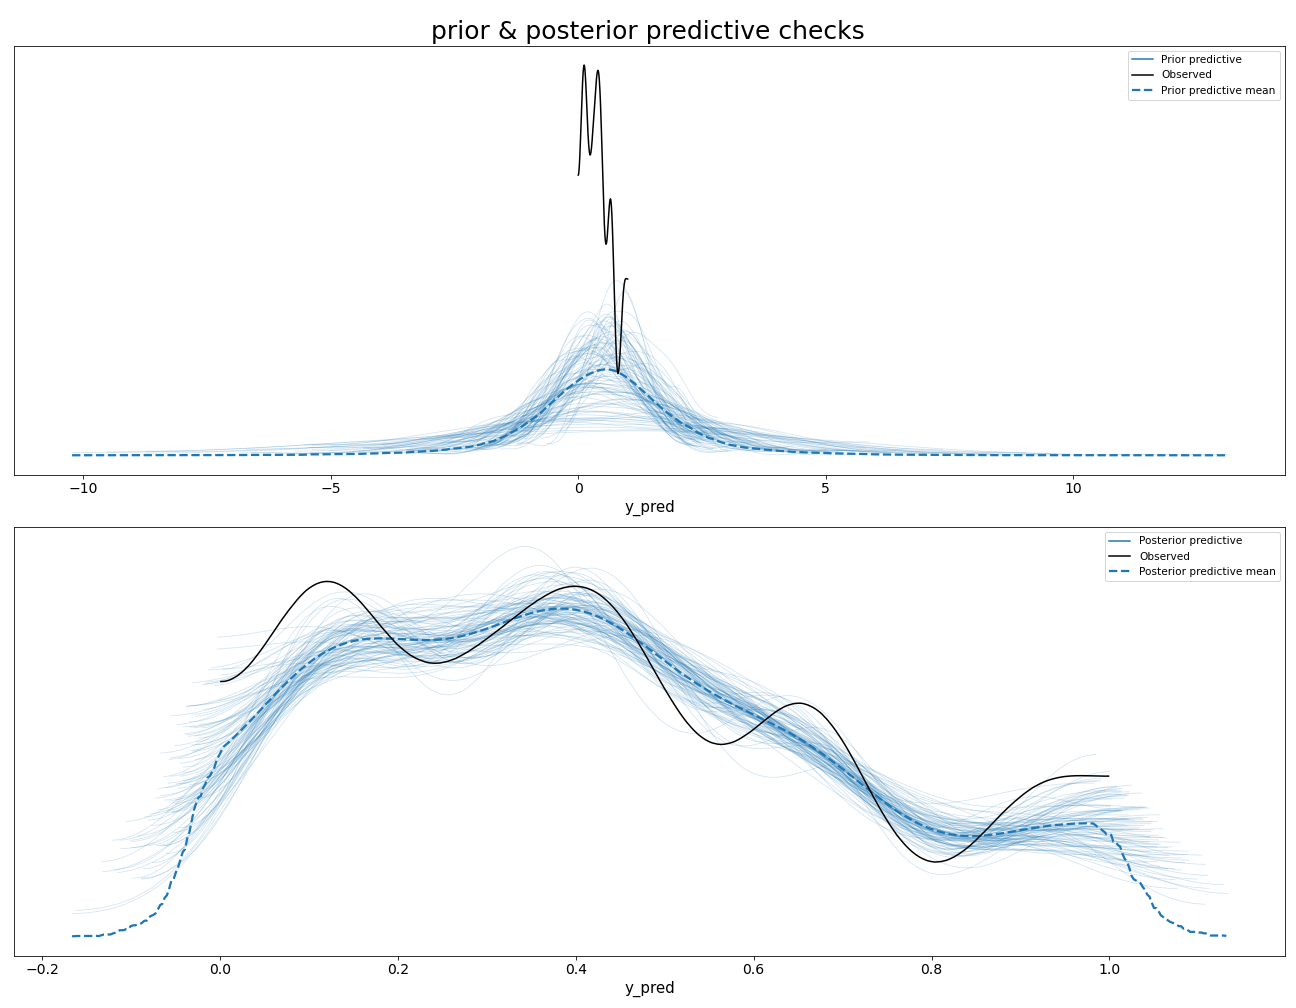
\includegraphics[width = 0.30 \textwidth]{../plots/ex1_second_plot_pp.png}}
    \subfigure[M3]{%
        \label{fig:supfigure3}
        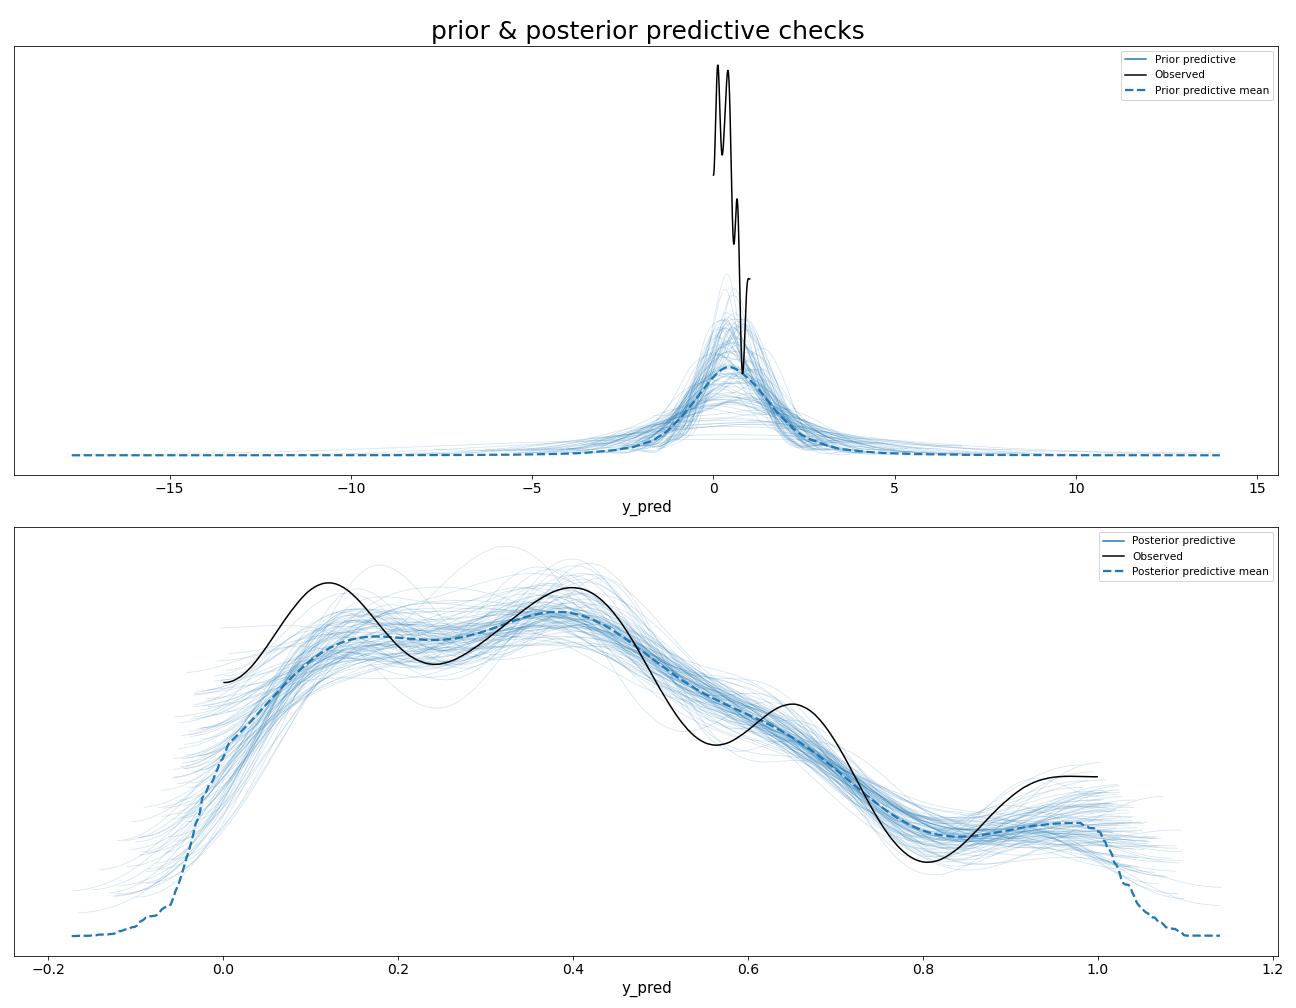
\includegraphics[width = 0.30 \textwidth]{../plots/ex1_third_plot_pp.png}}
    \quad
    \caption{Prior predictive and posterior predictive checks for the three models (M1, M2, M3) from left to right. Prior predictive checks at the top and posterior predictive checks at the bottom. Generated by PyCipio's plot\_pp() method which relies on PyMC3/Arviz backend.}
\end{figure}

When we look at the posterior predictive against the true (training) data, the overall picture is the same. For M1, the posterior predictive is reasonable, but it does miss some of the periodicity in the data. 
For M2, the posterior predictive fit to training data is almost perfect.
For M3 we see that the posterior predictive fit to the training data is pretty bad. 
More disturbingly, we see that the fit is qualitatively different for the two groups. 
It is smooth for "group\_one" and jagged for "group\_two". We believe that this is because of badly mixing chains, 
which are being averaged before making the plot. 

\begin{figure}[ht]
    \centering
    \subfigure[M1]{%
        \label{fig:supfigure1}
        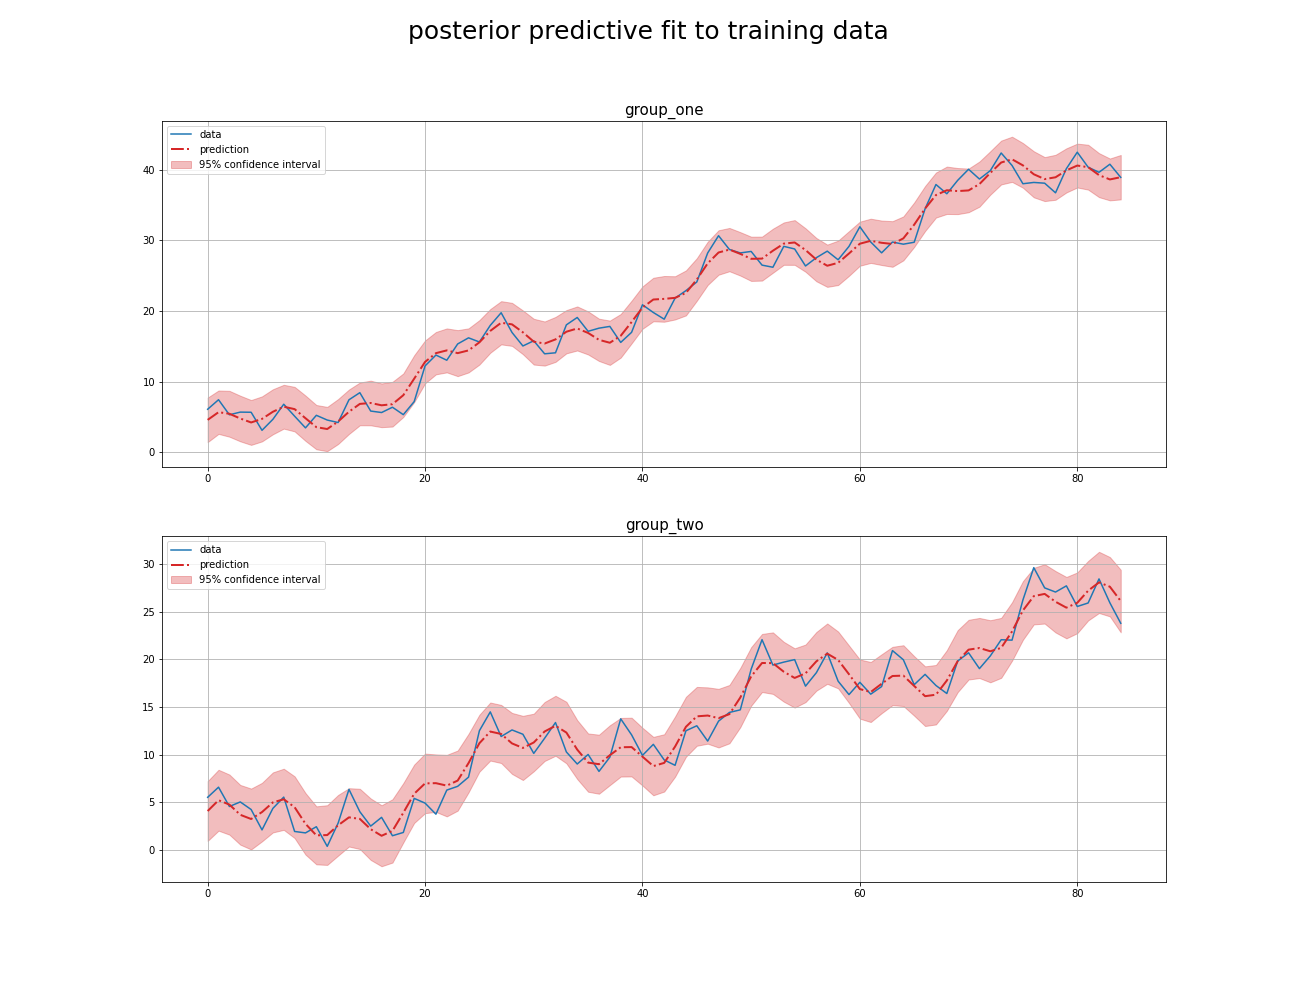
\includegraphics[width = 0.30 \textwidth]{../plots/ex1_first_plot_fit_idx_all.png}}
    \quad
    \subfigure[M2]{%
        \label{fig:supfigure2}
        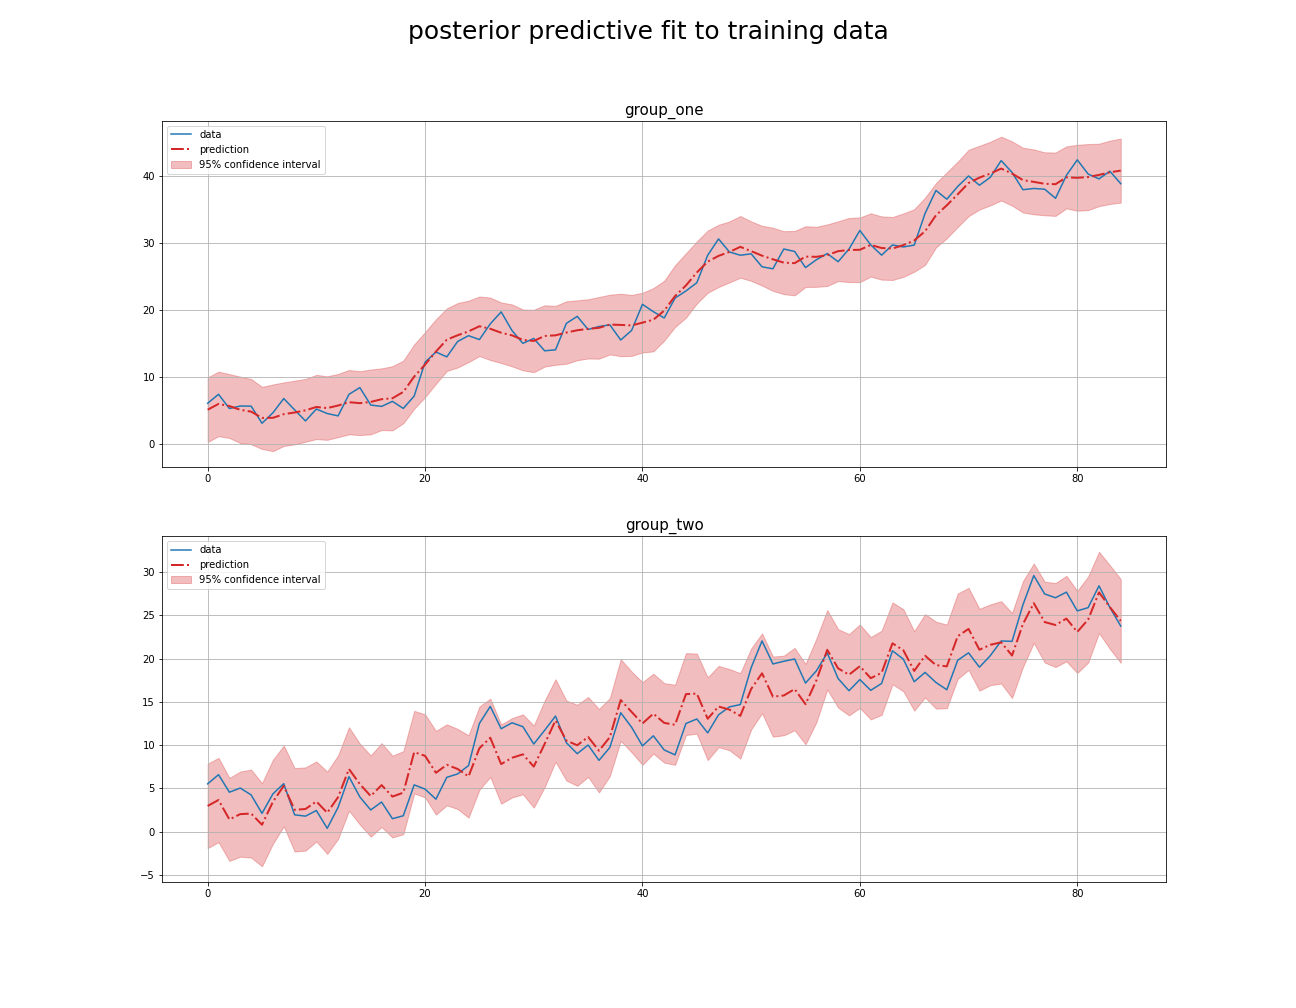
\includegraphics[width = 0.30 \textwidth]{../plots/ex1_second_plot_fit_idx_all.png}}
    \subfigure[M3]{%
        \label{fig:supfigure3}
        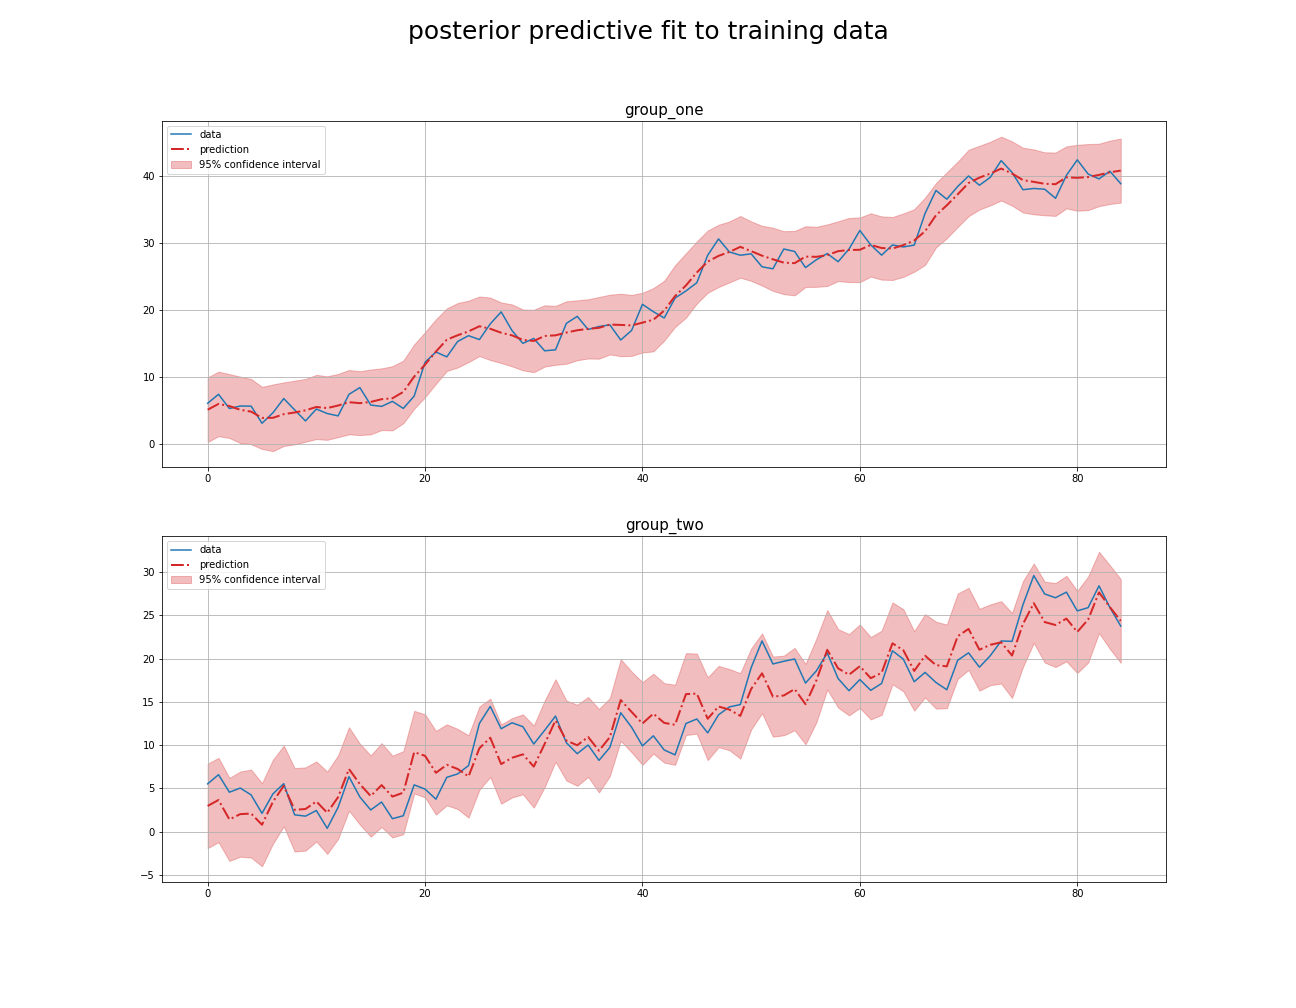
\includegraphics[width = 0.30 \textwidth]{../plots/ex1_third_plot_fit_idx_all.png}}
    \quad
    \caption{Posterior predictive checks (red) fit to training data (blue) for M1, M2 and M3 (left to right). For the first time-series fitted for each model at the top and for the second time-series for each model at the bottom. Shaded areas are 95\% prediction intervals. Generated by PyCipio's plot\_fit\_idx() method. }
\end{figure}

We now turn to predictions, and residual checks of the three models. Again we see that M1 does relatively well, and has a consistent accuracy across the two time-series. We see that M2 almost perfectly predicts the test data, and that M3 is problematic. The residual plots for M3 show clear patterns, and it is disturbing that M3 predicts one group much better than the other one. Clearly something has gone wrong with computation.  

\begin{figure}[H]
    \centering
    \subfigure[First plot]{%
        \label{fig:supfigure1}
        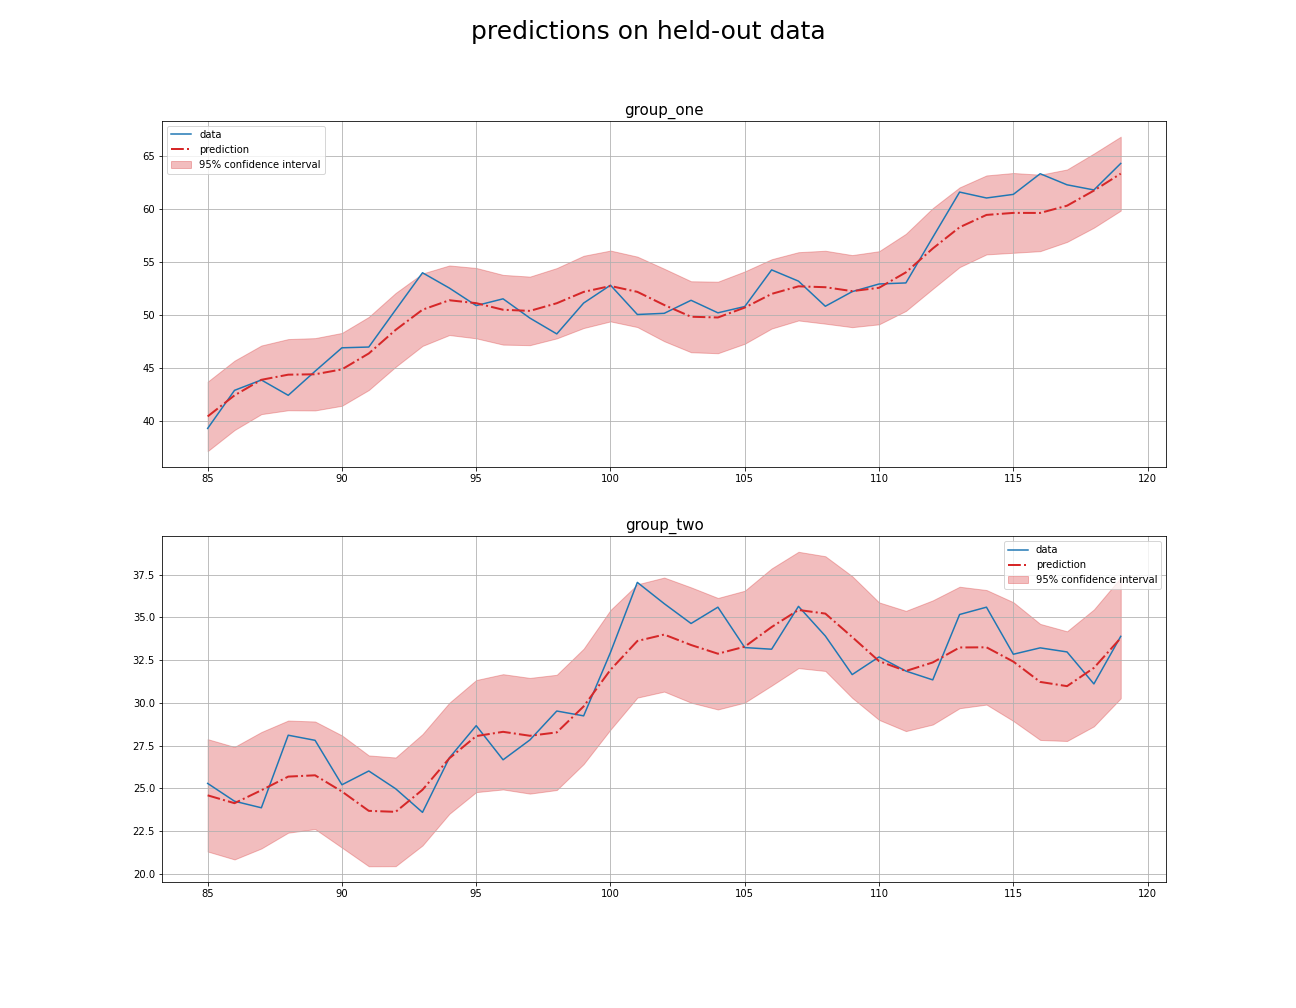
\includegraphics[width = 0.45 \textwidth]{../plots/ex1_first_plot_predict_idx_all.png}}
    \quad
    \subfigure[Second plot]{%
        \label{fig:supfigure2}
        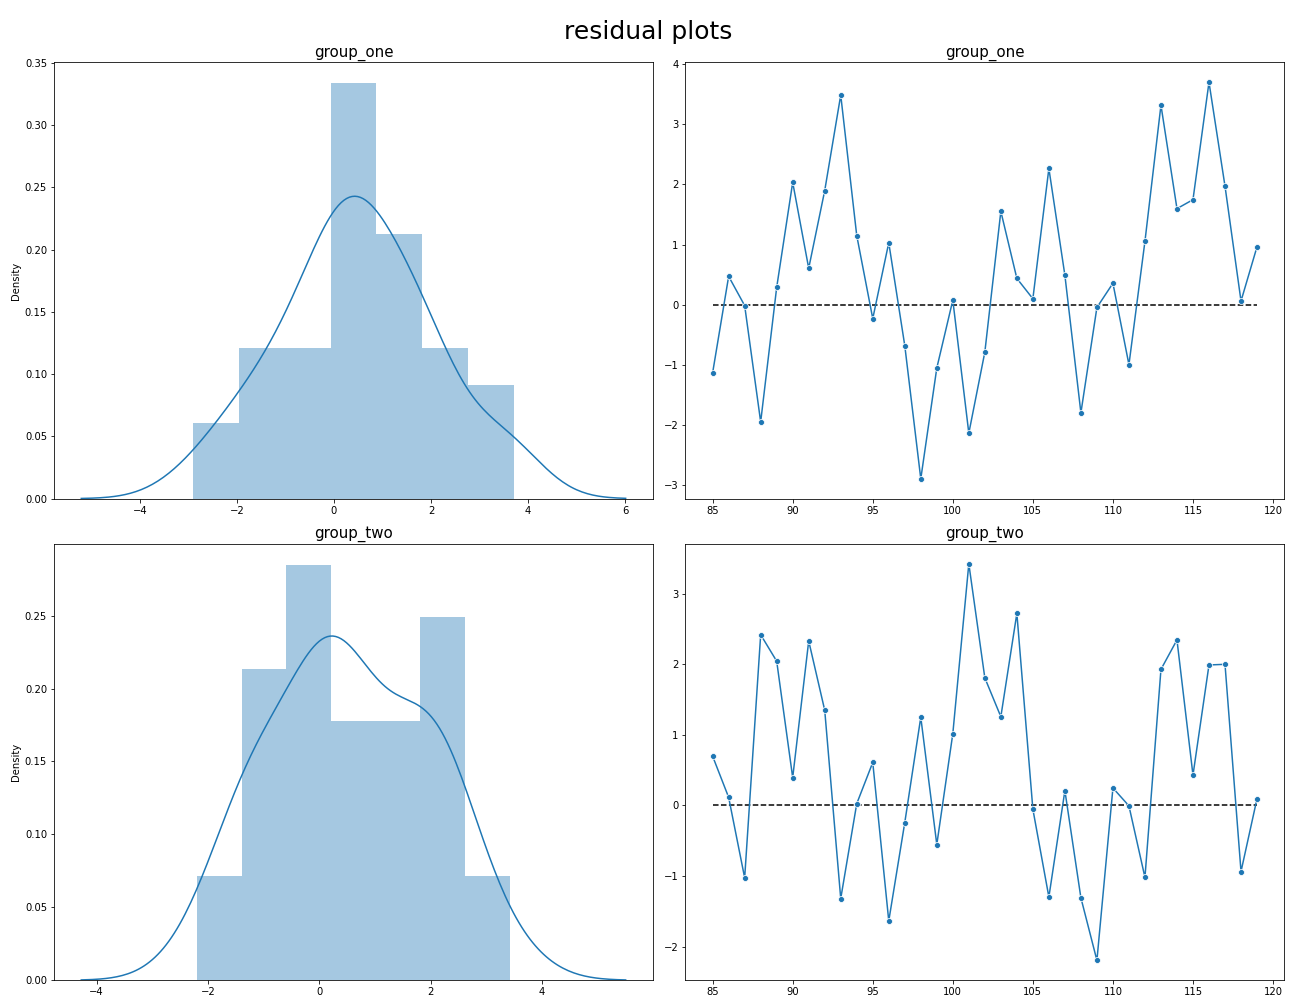
\includegraphics[width = 0.45 \textwidth]{../plots/ex1_first_residual_plots_all.png}}
    \subfigure[Third Plot]{%
        \label{fig:supfigure3}
        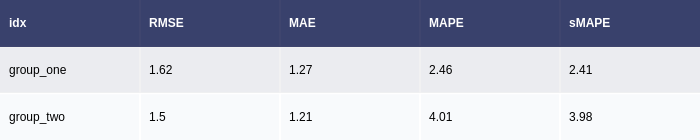
\includegraphics[width = 0.75 \textwidth]{../plots/ex1_first_get_errors.png}}
    \quad
    \caption{Top left: predictions (red) on unseen data and fit to this data (blue) with shaded 95\% uncertainty intervals for M1. Generated by PyCipio’s plot\_predict\_idx() method. Top right: KDE- and line-plot of residuals for M1 predictions on test data. Generated by PyCipio's plot\_residuals() method. Bottom: Forecast error indices for M1 generated by PyCipio's get\_error() method. In all plots, the top sub-plot corresponds to group\_one (first time-series) and the bottom sub-plot corresponds to group\_two (second time-series).}
\end{figure}
\begin{figure}[H]
    \centering
    \subfigure[First plot]{%
        \label{fig:supfigure1}
        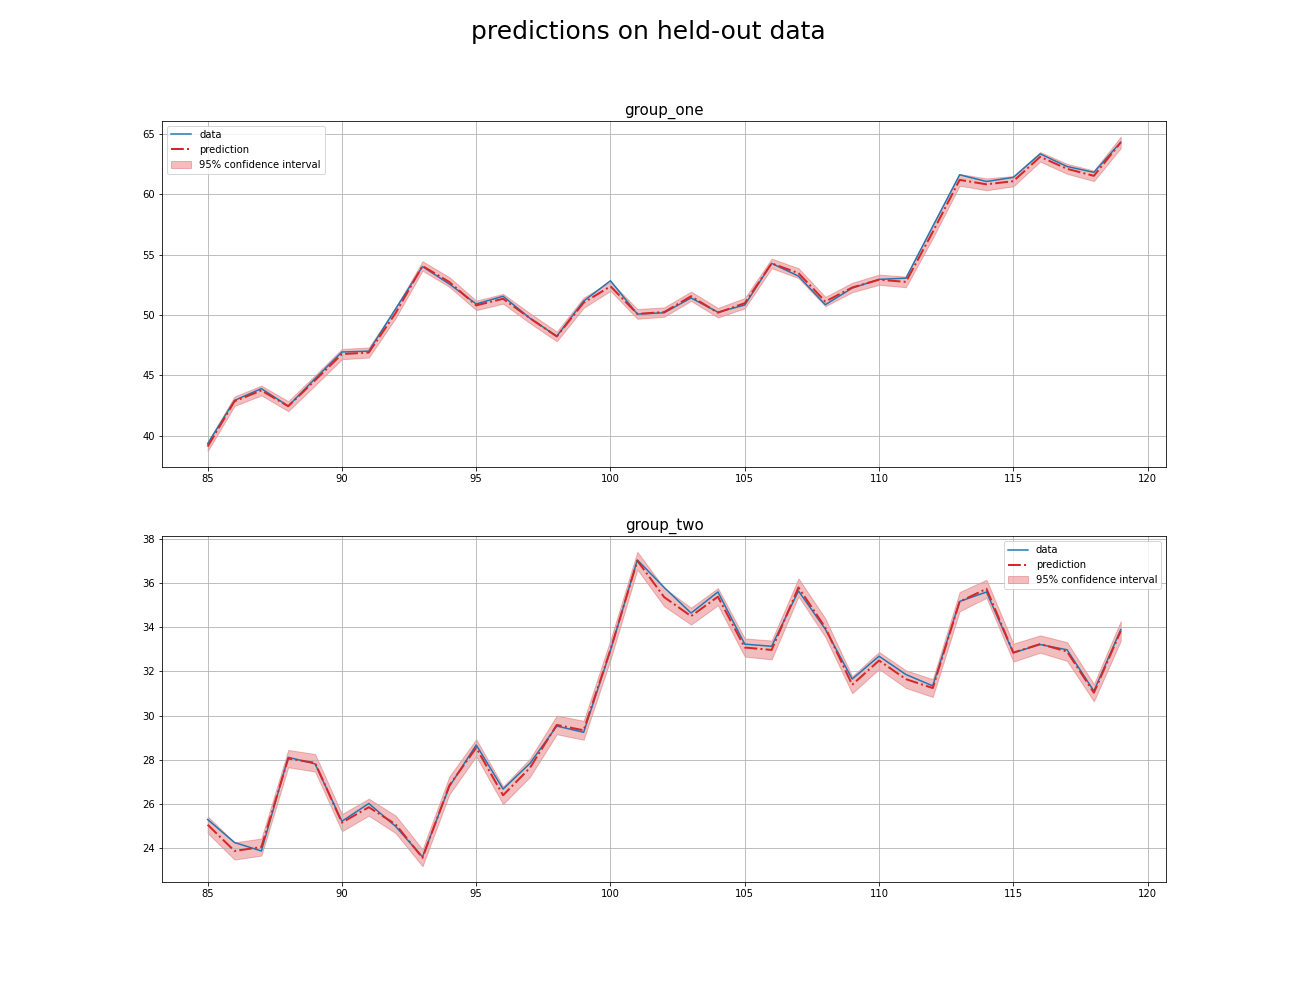
\includegraphics[width = 0.45 \textwidth]{../plots/ex1_second_plot_predict_idx_all.png}}
    \quad
    \subfigure[Second plot]{%
        \label{fig:supfigure2}
        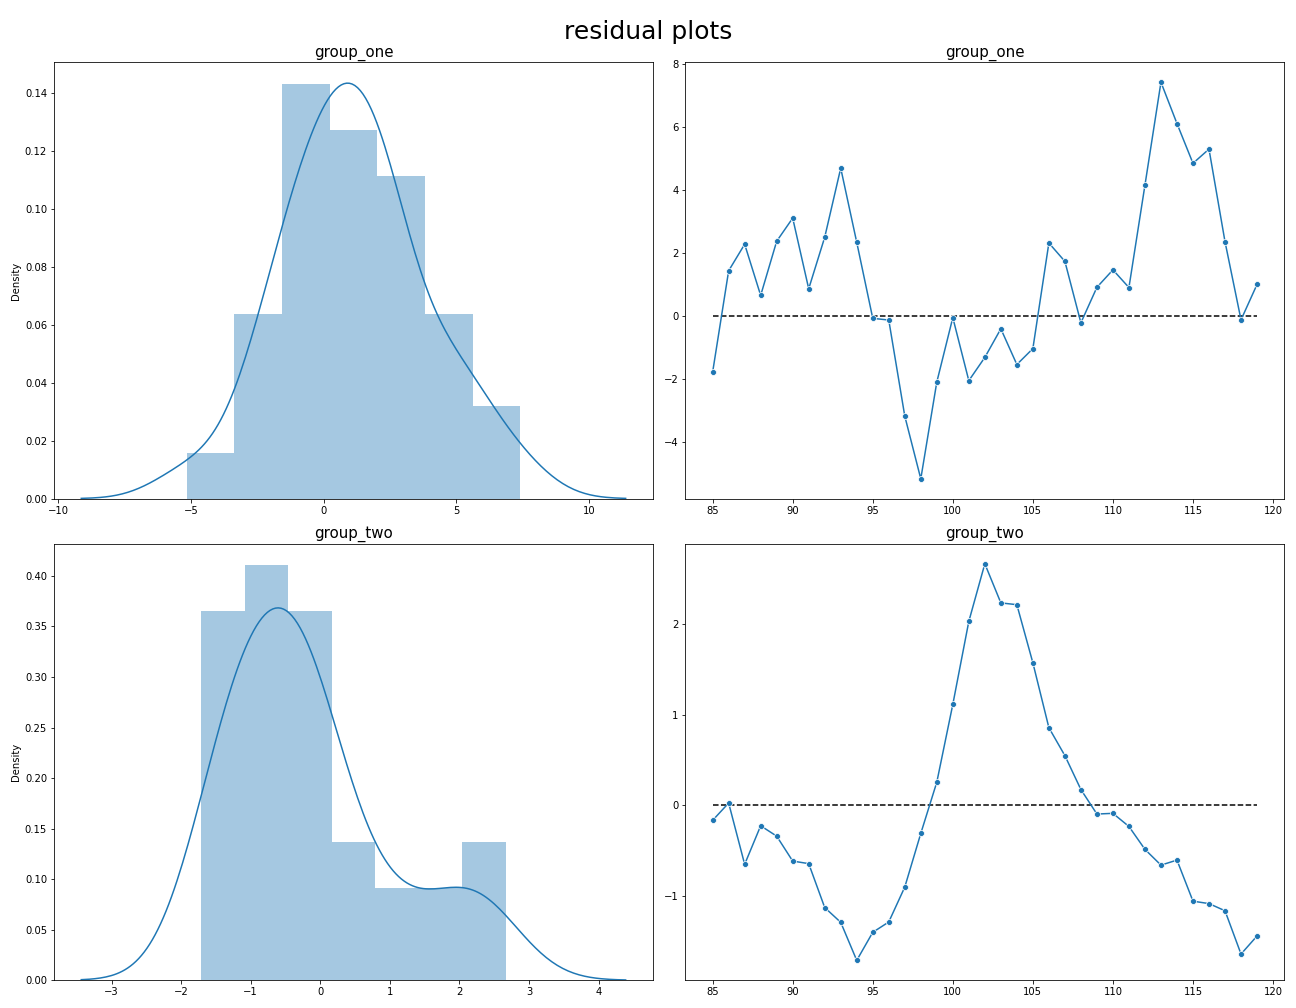
\includegraphics[width = 0.45 \textwidth]{../plots/ex1_second_residual_plots_all.png}}
    \subfigure[Third Plot]{%
        \label{fig:supfigure3}
        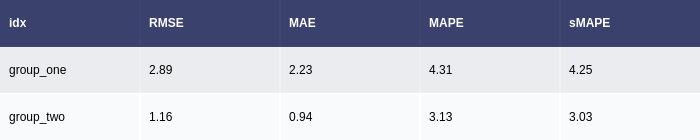
\includegraphics[width = 0.75 \textwidth]{../plots/ex1_second_get_errors.png}}
    \quad
    \caption{See description of figure above}
\end{figure}

\begin{figure}[H]
    \centering
    \subfigure[First plot]{%
        \label{fig:supfigure1}
        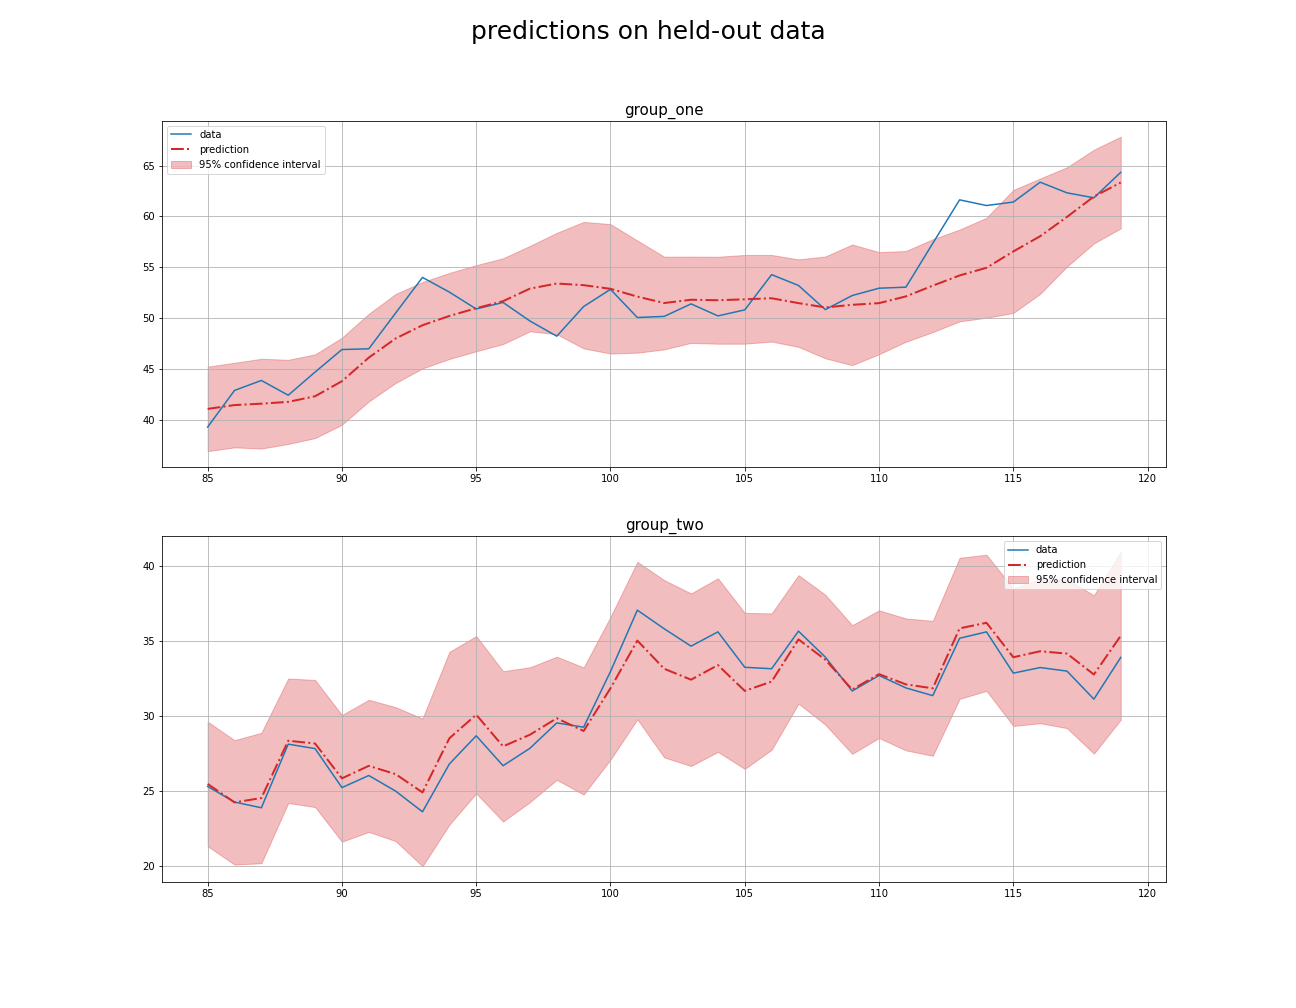
\includegraphics[width = 0.45 \textwidth]{../plots/ex1_third_plot_predict_idx_all.png}}
    \quad
    \subfigure[Second plot]{%
        \label{fig:supfigure2}
        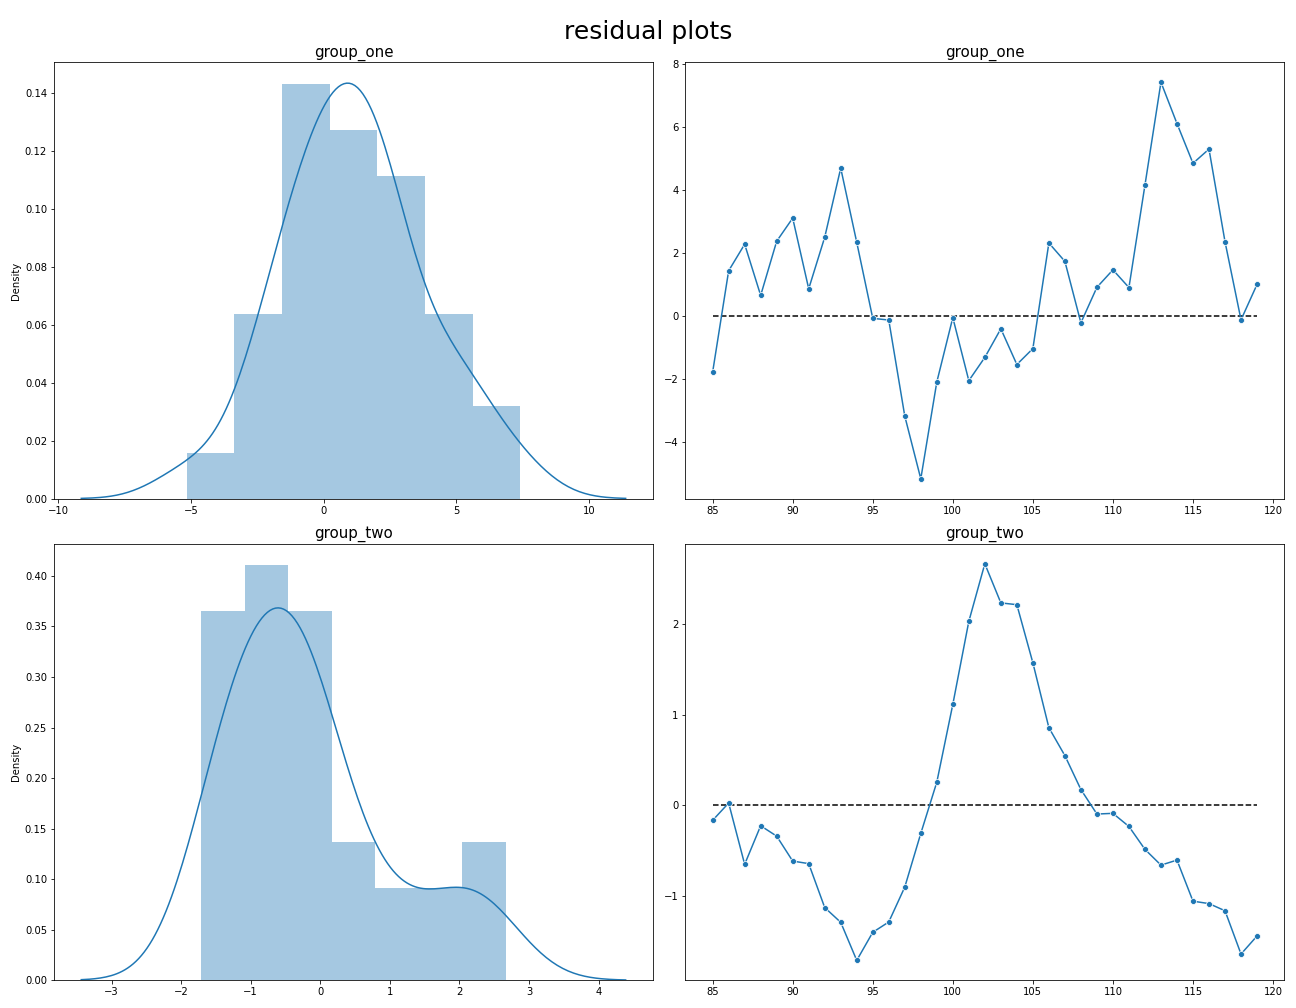
\includegraphics[width = 0.45 \textwidth]{../plots/ex1_third_residual_plots_all.png}}
    \subfigure[Third Plot]{%
        \label{fig:supfigure3}
        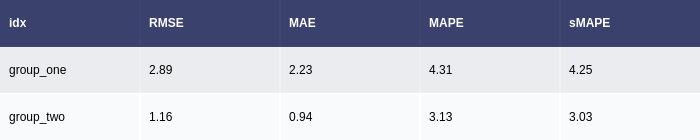
\includegraphics[width = 0.75 \textwidth]{../plots/ex1_third_get_errors.png}}
    \quad
    \caption{See description of figure above}
\end{figure}

In sum, we see three different patterns for the three different models that we have fit in this toy example. For an underfit model, we see reliable estimation of parameters and prediction. I.e., the posterior predictive fit to data, and the prediction errors for the two time-series are approximately equal for M1. However, an underfit model will miss reliable components of the data and as such is suboptimal. 

We see that the overfit model is especially problematic. The chains do not converge, which we originally thought was because there are multiple ways that the model can fit the data equally well. While this is certainly the case, there is an additional issue. The sigma (from the rightmost trace-plot) shows that one chain has a much larger error than the other one. Something is not working properly in the computation, but we are not exactly sure what breaks and whether it is something that can be optimized, or is more fundamentally wrong. 

The model with appropriate complexity fits and predicts the data extremely well. Of course, this is a result of the data being generated from components that our model is designed to be able to fit (i.e. sine- and cosine waves, intercept and linear trend). However, this is still a comforting sanity check to our framework.

We note that the periods are slightly different for the two time-series, but because we estimate our periods (here with priors around 7 \& 30) we are able to fit periods which are not exactly identical across these two time-series. This is obviously not possible for frameworks which use a hard-coded periodic component (e.g. Prophet). 

\subsection{Example 2}

For our second example, we try to model alcohol sales over the course of several years (1992 - 2019). As the data only has one group, we are here showcasing the functionality of single group predictions. The data is a monthly time-series, which shows a clear linear trend across most, but not all of the time series. In addition, it has a clear yearly seasonality. The amplitude of this yearly seasonality increases as a function of time, and it therefore makes sense to use a multiplicative seasonality component.

\begin{figure}[H]
    \centerline{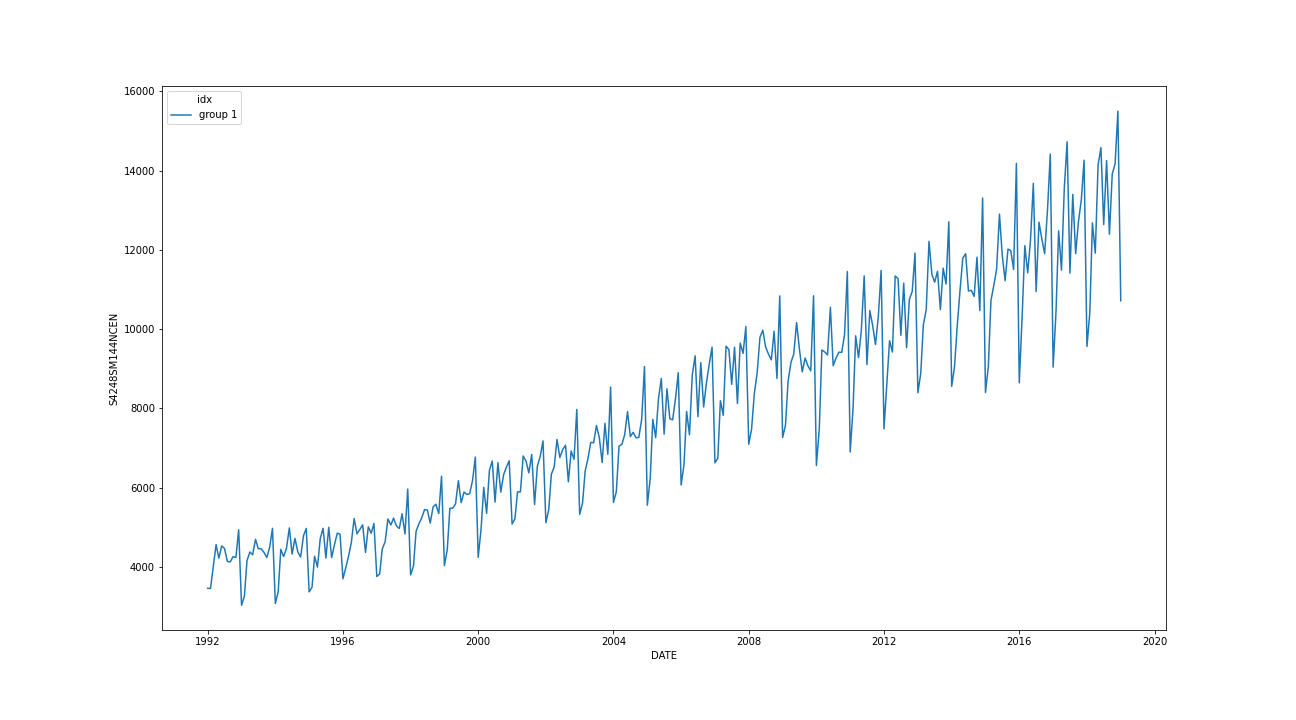
\includegraphics[scale = 0.45]{../plots/ex2_plot_data.png}}
    \caption{Seaborn line plot of the alcohol sales. Generated with the plot\_data() method from PyCipio. }
\end{figure}

First thing to note is that not all of the data show a clear linear trend (see Fig X). The very beginning of the time-series (from 1992 to 1995) does not seem to have any trend at all. Based on the exploratory visualization (above) we set the priors for the seasonal components to (4, 4) and (12, 6) where the first is additive and the second is multiplicative. In this example we will jump straight to the predictions from the model. 

\begin{figure}[H]
    \centering
    \subfigure[First plot]{%
        \label{fig:supfigure1}
        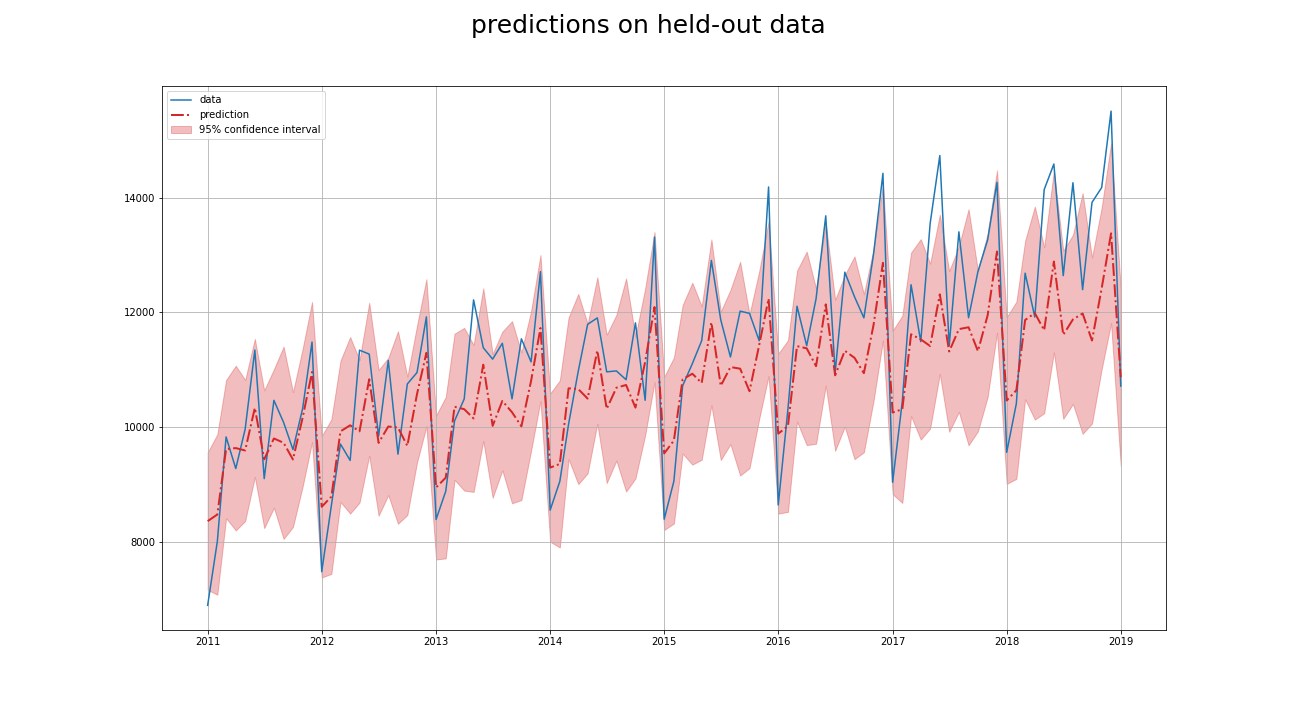
\includegraphics[width = 0.75 \textwidth]{../plots/ex2_plot_predict_idx_full.png}}
    \quad
    \subfigure[Second plot]{%
        \label{fig:supfigure2}
        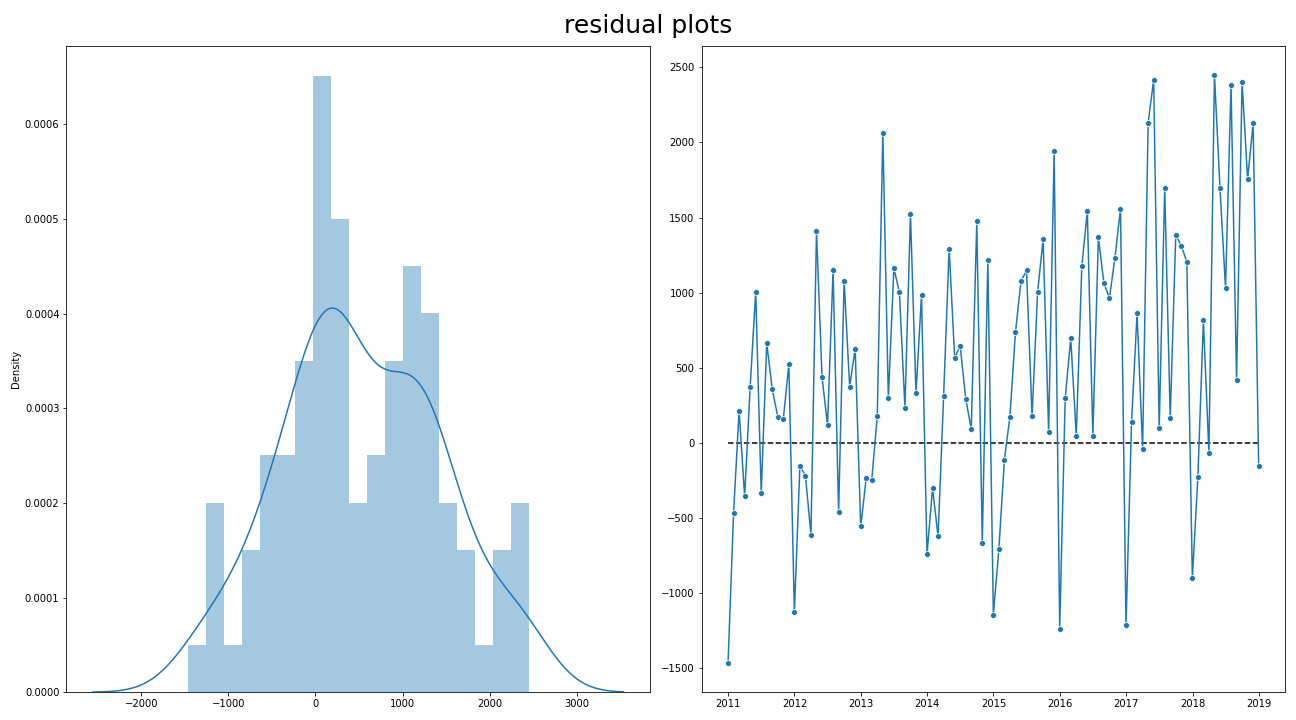
\includegraphics[width = 0.75 \textwidth]{../plots/ex2_plot_residuals_full.png}}
    \subfigure[Third Plot]{%
        \label{fig:supfigure3}
        
\includegraphics[width = 0.75 \textwidth]{../plots/ex2_get_errors_full.png}}
    \quad
    \caption{All plots for the model trained on the full training data for alcohol sales data set. (top row) predictions on held-out data. Blue line is the test data, red line is the point estimate (mean) of the posterior predictive and shaded areas are 95\% prediction intervals. (middle row) residual plots with KDE to the left and line-plot to the right. (bottom row): Forecast error indices. }
\end{figure}

From inspecting the predictions, we can see that our estimation of $p$ seems to be a good fit to the test data. However, our predictions consistently undershoot the actual values, which appears to worsen over time. This systematic issue is clear in the residual plots as well. Firstly, the residuals are not normally distributed, and are not centered around 0, which we would ideally like. We can also see from the residual plot over time (to the right) that this bias gets worse over time. This could be explained by the lack of a linear trend in the first years of the data. As the trend component in the model is estimated globally on the training data, the lack of a trend in the beginning will result in our model undershooting the value of $\beta$, the slope of the linear model. 

One way of checking whether this is a correct diagnosis of the problem is by removing the first couple of years in the training data. We therefore delete all data points from before 1995, and rerun the model with the same settings.


\begin{figure}[H]
    \centering
    \subfigure[First plot]{%
        \label{fig:supfigure1}
        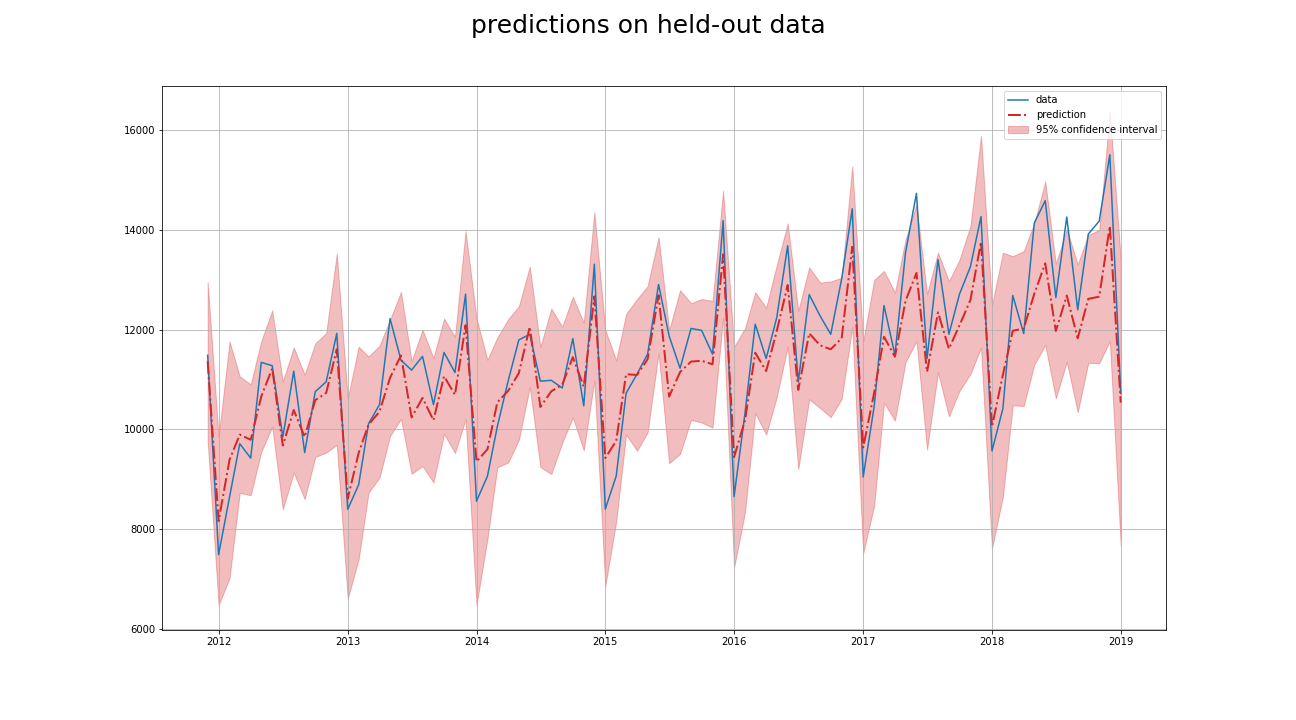
\includegraphics[width = 0.75 \textwidth]{../plots/ex2_plot_predict_idx_crop.png}}
    \quad
    \subfigure[Second plot]{%
        \label{fig:supfigure2}
        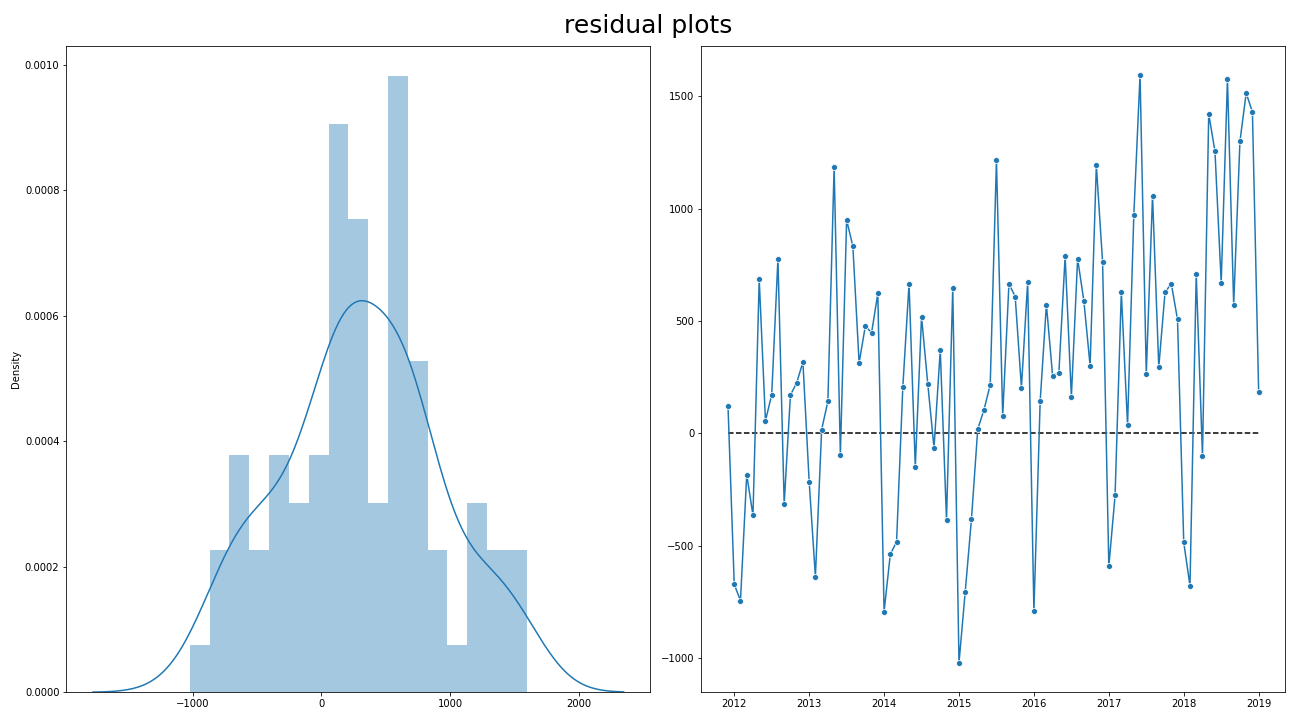
\includegraphics[width = 0.75 \textwidth]{../plots/ex2_plot_residuals_crop.png}}
    \subfigure[Third Plot]{%
        \label{fig:supfigure3}
        
\includegraphics[width = 0.75 \textwidth]{../plots/ex2_get_errors_crop.png}}
    \quad
    \caption{All plots for the model trained on a subset of alcohol sales data. (top row) predictions on held-out data. Blue line is the test data, red line is the point estimate (mean) of the posterior predictive and shaded areas are 95\% prediction intervals. (middle row) residual plots with KDE to the left and line-plot to the right. (bottom row): Forecast error indices. }
\end{figure}

The model which is fit on a subset of the data still undershoots the trend, but the error is much lower compared to the model fit on the full training data. One way of seeing this is by noticing that the scales in the plots are different, and that the forecast error indices are much lower for this second model. So although omitting the first part of the time-series does not fix all the model's problems, it increases its test accuracy significantly. 

In sum this example shows that PyCipio can model some real-world data with clear patterns relatively well. It does indicate that we lack an implementation for discounting early observations, or relatedly give more weight to recent observations. 

\subsection{Example 3}

The two previous examples have dealt with either simulated data that exhibit clear patterns or real-world sales data that similarly behaves relatively well. This third example uses real-world COVID-19 data to highlight a problematic case. The data was obtained from the COVID-19 data hub API \cite{COVID-19-data-hub}, which globally accesses governmental sources at national, regional, and city level providing various COVID-related metrics. For demonstrational purposes, we selected a subset of four states in USA (Florida, Nevada, California, and Texas) and daily covid metrics spanning from March 2020 to May 2021. Because of changes in how and when COVID numbers have been recorded, a rolling average window (width = 3 days) was used to smooth the time series. This had the additional merit of taking care of the few cases of missing data. Moreover, the data was scaled to "new infected pr. 100k captita" to account for vast differences in state populations and their COVID numbers.  

\begin{figure}[H]
    \centerline{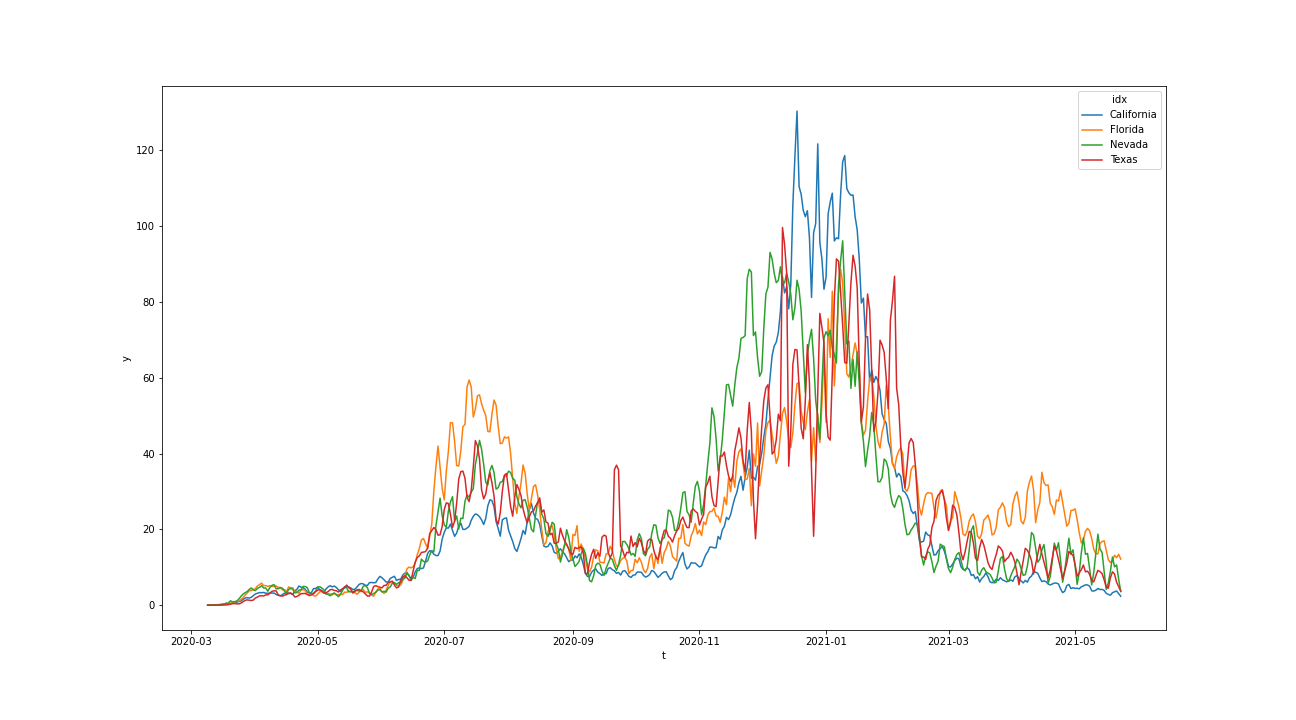
\includegraphics[scale = 0.45]{../plots/ex3_raw_data.png}}
    \caption{Line plot of COVID data from 4 states. Daily new infected pr. 100k capita.}
\end{figure}

As can be seen from the plot, this is a problematic case as the time series exhibit no clear linear trend. Moreover, there is no obvious recurring periodicity. COVID cases are a difficult time-series forecasting scenario, both generally and for PyCipio. COVID cases have been successfully modelled in more advanced settings, but it is difficult when we restrict ourselves to only use time as a predictor. Most prominently, we see the impact of the first and second wave of the pandemic occurring simultaneously in all four states. Had the pandemic been a recurring event stretching over multiple years, these waves could potentially be accounted for as some semi quarterly seasonality. We chose priors (7, 1) for the first seasonal component, and (75, 1) for the second seasonal component. The (7, 1) seasonal component is multiplicative, while the (75, 1) seasonal component is additive. 

\begin{figure}[H]
    \centering
    \subfigure[First plot]{ %did it work?
        \label{fig:supfigure1}
        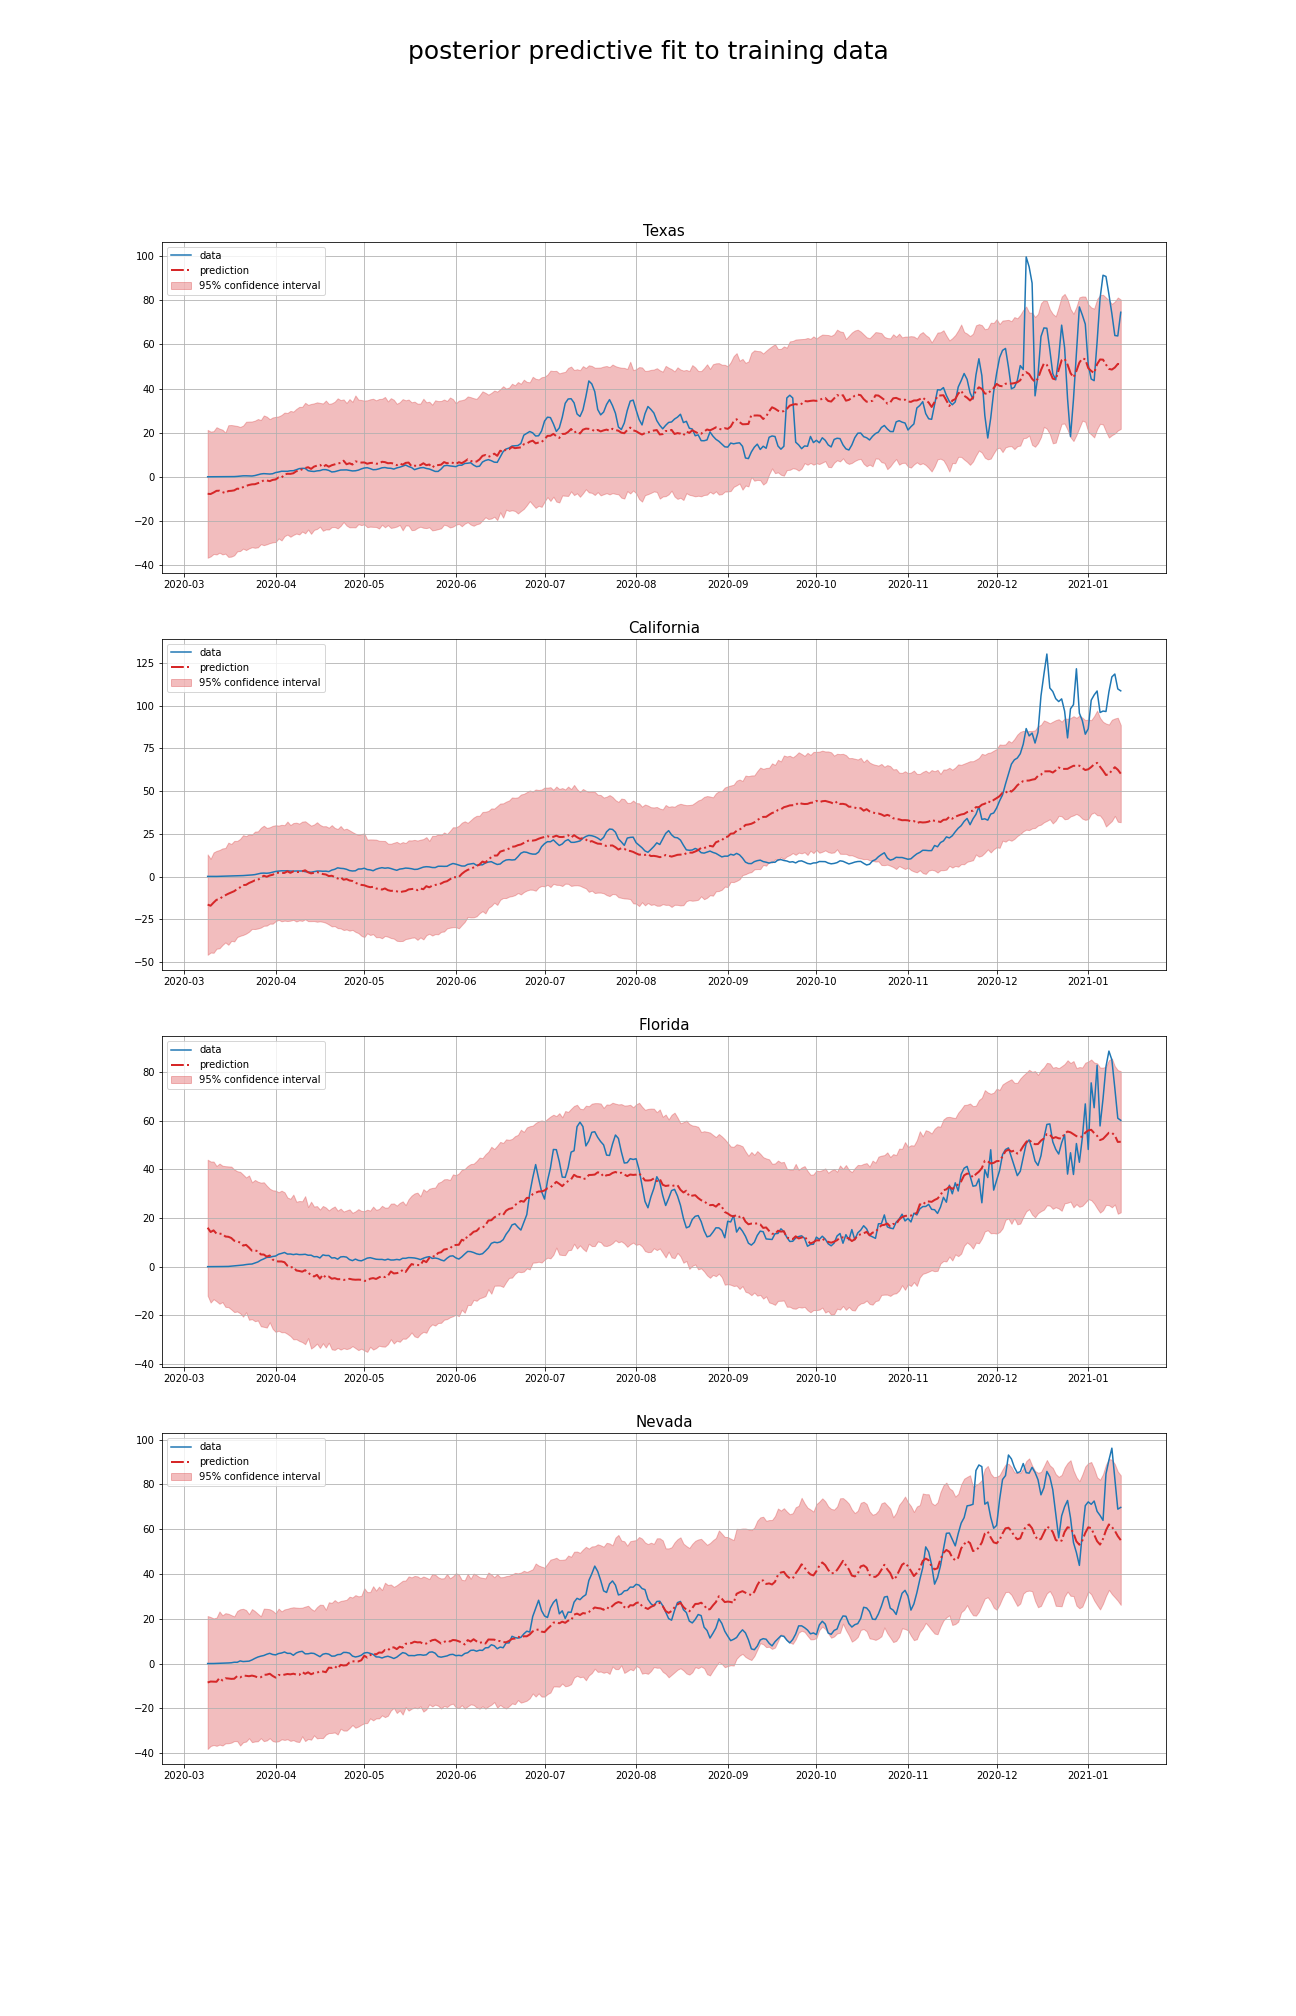
\includegraphics[width = 0.45 \textwidth]{../plots/ex3_plot_fit_idx.png}}
    \quad
    \subfigure[Second plot]{%
        \label{fig:supfigure2}
        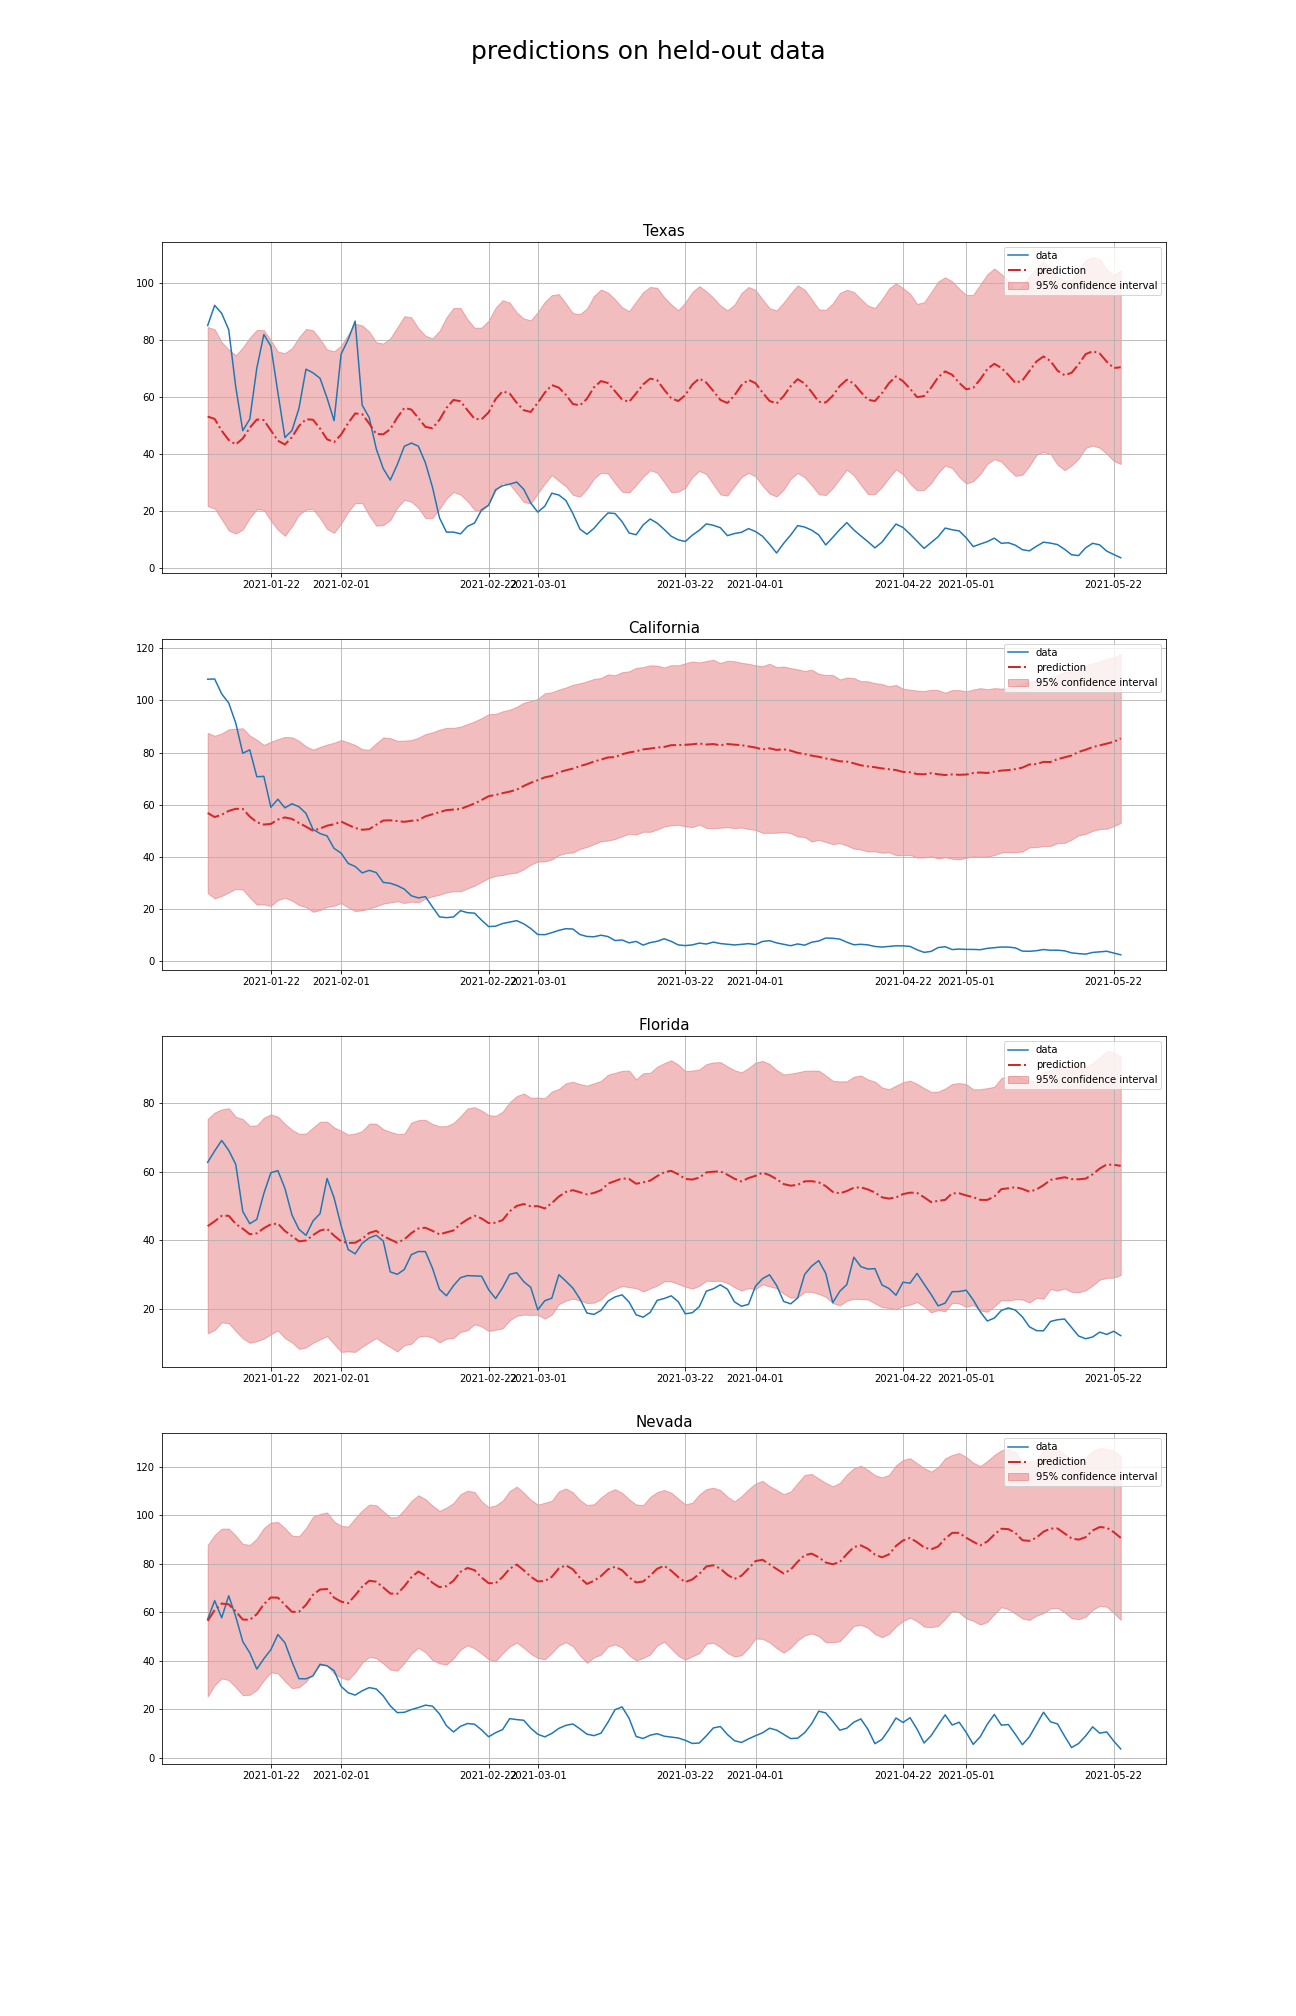
\includegraphics[width = 0.45 \textwidth]{../plots/ex3_plot_predict_idx.png}}
    \caption{(left) Posterior predictive checks (red) against training data (blue). From top to bottom, Texas, California, Florida and Nevada. Shaded regions are 95\% prediction intervals. (right) Predictions on unseen test data (red) against test data (blue). From top to bottom, Texas, California, Florida and Nevada. Shaded regions are 95\% prediction intervals. }
\end{figure}

In plot (A), we see somewhat reasonable posterior predictive fits to training data for Texas and Florida. For instance, the periodicity of the longer period for Florida (around 5 months) seems to be accurate, as well as the linear trend. We do see worse fits for California and Nevada. 

Despite some of the states having relatively reasonable posterior predictive fits to the data, we see that the predictions for all states are off by a large margin. It is noteworthy that the new cases drop for all states almost exactly at the split between test and train data. Our model (a) has no way of knowing that this will happen and (b) does not have the flexibility to model this. 

What we would need in order to model COVID cases is something like the holiday component which Facebook Prophet offers, or including knowledge outside of the time-series (e.g. that we know that new restrictions will take effect). 

In sum, none of our components really capture a reliable and repeating pattern in the data. This is because there are no recurring patterns in the data. 


\section{Related work and differences}

In creating PyCipio we have tried to merge the best from multiple other sources. These include the \textit{"Forecasting: Principles and Practice (FPP3)"} time series forecasting framework \cite{fpp3} and Facebook Prophet \cite{taylor2018forecasting}.

We drew inspiration from FPP3’s general modeling workflow and their focus on residual diagnostics. 

In FPP3, forecasting begins with some time series data in the tsibble format. This is a data- and model-oriented object which preserves time indices as the essential data column, allowing for an easy transition between data loading, preprocessing, modelling and eventually generating predictions. PyCipio aims to offer a similarly accessible modelling approach. 

Some of the residual diagnostics and visualizations demonstrated in FPP3 are implemented in the PyCipio class, as these offer an efficient method for assessing the quality of a model.
The kernel density estimate (KDE) plot of residuals allows for a quick assessment of whether the residuals are mean centered at 0, indicating if a bias is present in the model. The line plot of residuals allows for the visual inspection of autocorrelation and systematicity between residuals. This expresses the extent to which there is unmapped signal left in the data that could be modelled to improve model fit and predictive power \cite{fpp3}. This was the case in our second example (Alcohol sales) where the KDE residuals were not centered around 0 and the residuals over time showed systematic variance. 

Inspired by \textit{"Facebook Prophet"}, we use the exact same method of Fourier Series decomposition for the seasonal component. The general design philosophy of Facebook Prophet with including the "analyst-in-the-loop" instead of automating time-series prediction is also a part of our intended workflow \cite{taylor2018forecasting}. 
Facebook Prophet does not estimate the period (p) length of their seasonal components, which is a point of difference. Estimating p is often useful, as the user might have a rough estimate of the period of a seasonal component without knowing the exact value. Facebook Prophet also includes a holiday component in their decomposition. This is a very useful feature for some time-series cases, and it could potentially have been useful in our third example regarding COVID. We would be able to model the summer holiday as well as Christmas as separate components. Incidentally, these are the two periods where the time-series are most volatile.


\section{Limitations and future work}

\subsection{The Goal of PyCipio}

Our goal for PyCipio was developing a time-series forecasting tool which merges the powerful inference engine from PyMC3 with the ease of getting predictions from scikit-learn. In some ways, we achieved our goal for the package. For instance, the same pipeline can be used to model very different data, as shown in our examples. However, there are still several key points where the package could be either expanded or tweaked. Most of them revolve around getting the benefit of implementing a full Bayesian model, which allows for more advanced features that are not currently a part of the package. These include flexibility in model specification, hierarchical modelling and predictions into the future without having a test-set. 


\subsection{Flexibility}

One of the main advantages of a Bayesian model specification is that domain knowledge can be used to set reasonable priors which makes for better models \cite{McElreath}. While the priors for the seasonal component are adjustable in the current implementation of PyCipio, the priors for the trend component (i.e. $\alpha$ and $\beta$) are hard-coded. It is possible for us to set reasonable broad priors for these parameters because we min-max scale both $x$ and $y$. However, an improved version of PyCipio would allow for (a) using default priors or (b) specifying priors on the natural scale of the data which we then scale with the data. 

PyCipio applies min/max-scaling to both $y$ and $x$ values in the time series during model fitting. This occurs “behind the scene” and is applied across groups on the training data whilst carrying scaling values over to the test data. Scaled values typically make sampling easier which ensures robust parameter estimation. The values can easily be scaled back after model fitting, which also occurs automatically in PyCipio. This scaling simply ensures that variables that are measured across different scales can contribute equally to the fit of the model \cite{Min-Max}. 

Additionally, the current implementation only supports a linear model of the data. However, trends are often not linear. Common examples are exponential trends or polynomial trends. Just by including these two types of trends in the model, the generalizability of PyCipio would greatly increase. As noted previously, the trend component also weights all data points equally. This strong assumption is very often wrong in time-series, where less recent points should be discounted. 

\subsection{Hierarchical}

One thing we did not implement in PyCipio yet is the option to do multilevel modeling (also commonly referred to as random effects models).

There are several advantages to multilevel modeling, including accounting for hierarchical structure of the data, better parameter estimation for underrepresented groups, and better estimation of group-level effects \cite{Fonnesbeck}. Multilevel models are a natural way to balance the overfitting/underfitting trade-off by means of partially pooling estimates \cite[p.~14]{McElreath}. This leads multilevel models to make better estimates on average \cite[p.~414]{McElreath}.

Multilevel modeling for time-series forecasting could be useful in cases where we have clusters of data, such as in example 3. Here we have US states, each of which can be thought of as a random variable drawn from a distribution over the population of US states. Our current workflow supports two ways of dealing with this data. Either, the user could pre-average the data from all the states, in order to model and predict COVID cases for the US as a whole. Alternatively, the user could model all the states (or a subset) individually, as we did in our example analysis.

The first approach, which averages all the data, is problematic because it throws away data and will be too insensitive. It will thus be underfit, and it will also be overly optimistic with regards to uncertainty (i.e. we are not incorporating all levels of uncertainty).

The second approach can be valid if we do not believe that the states share a significant portion of their variance (say e.g. that the states decide on their own policy with regards to social distancing). Most likely however, the states will share some variance because they share some cultural norms, some legislation or that people can move between states and bring COVID with them. By modeling the states individually, we are forcing the model to treat the states as completely separate entities and telling it that it can learn nothing about the possible values of new infections in California by observing what is happening in Texas. This will lead to overfitting to each sample (i.e. each state).

\subsection{Prediction on unseen data set}

In the current build of PyCipio, users can't forecast into the future. This is because PyCipio takes a dataframe as input and splits it into a training and test set, fits the model on the training data, and then makes predictions based on the test data. PyCipio does not predict outside of this test set. This is adequate for tuning your model and running diagnostics. However, this fails to apply to a real-world time series forecasting scenario. Ideally, users would be able to fit and tune their model on the training data, run diagnostics on some held-out test data, and then run the model forward into future time steps as specified by a horizon parameter. This is how a time series modelling and forecasting framework would actually be applicable in say, a business setting, as it would allow users to generate specific predictions that aligned with their specific forecasting goal and context.

\section{Conclusion}

This paper has introduced PyCipio which aims to provide the python community with a package that facilitates easy implementation of bayesian time-series forecasting. The package aims to do so while retaining some of the flexibility and control that is possible within a Bayesian modeling context. The package works by decomposing a signal into seasonal components and a linear trend. We have demonstrated the cases in which these components can meaningfully predict data, and the cases in which the current functionality is not sufficient. The package relies on the pyMC3 backend, and draws inspiration from other time-series frameworks, such as Facebook Prophet. As the focus of the package has been to provide the user with an easy way of conducting time-series analysis, the package is not well suited for other Bayesian modeling tasks, such as inference and parameter estimation. 

\bibliographystyle{apacite}

\bibliography{../Referencer_new}

\end{document}